\documentclass[msc]{ppgccufmg}    % ou [msc] para disserta��es
                                  % de mestrado. Para propostas ou
                                  % projetos, usar [phd,project],
                                  % [msc,proposal], etc.

\usepackage[english]{babel}       % se o documento for em ingl�s
\usepackage[latin1]{inputenc}
\usepackage[T1]{fontenc}
\usepackage{type1ec}
\usepackage[a4paper,
  portuguese,
  bookmarks=true,
  bookmarksnumbered=true,
  linktocpage,
  colorlinks,
  citecolor=black,
  urlcolor=black,
  linkcolor=black,
  filecolor=black,
  ]{hyperref}
\usepackage[square]{natbib}

\usepackage{adjustbox}
\usepackage{array}

\newcolumntype{R}[2]{
    >{\adjustbox{angle=#1,lap=\width-(#2)}\bgroup}
    l
    <{\egroup}
}
\newcommand*\rot{\multicolumn{1}{R{45}{1em}}}

\usepackage{booktabs} % For formal tables
\usepackage[ruled]{algorithm2e} % For algorithms
\renewcommand{\algorithmcfname}{ALGORITHM}
\SetAlFnt{\small}
\SetAlCapFnt{\small}
\SetAlCapNameFnt{\small}
\SetAlCapHSkip{0pt}
\IncMargin{-\parindent}

\usepackage{graphicx}
\usepackage{mathtools}
\usepackage{amsfonts}
\usepackage{amsmath}
\usepackage{multirow}
\usepackage[cal=boondox]{mathalfa}
\usepackage{pgfplots}

\usepackage{tikz}
\usetikzlibrary{arrows,automata}

\DeclareMathOperator*{\argmax}{arg\,max\,}
\renewcommand{\arraystretch}{1.2}

\usepackage{filecontents}

\begin{document}

\ppgccufmg{
  title={Web data extraction through named entity labeling},
  authorrev={de Freitas Veneroso, Jo�o Mateus},
  cutter={D1234p},
  cdu={519.6*82.10},
  university={Federal University of Minas Gerais},
  course={Computer Science},
  portuguesetitle={Extra��o de dados da web por rotulamento de sequ�ncias},
  portugueseuniversity={Universidade Federal de Minas Gerais},
  portuguesecourse={Ci�ncia da Computa��o},
  address={Belo Horizonte},
  date={2019-07},
  advisor={Berthier Ribeiro-Neto de Ara�jo},
  approval={pics/approvalsheet.eps},
  abstract=[brazil]{Resumo}{resumo},
  abstract={Abstract}{abstract},
  dedication={dedicatoria},
  ack={agradecimentos},
  epigraphtext={Truth and lie are opposite things.}{Unknown},
  keywords={Vis�o Computacional, Redes, Sabotagens},
}

\chapter{Introduction}

HTML documents most often lie in between the structured/unstructured 
data paradigm. DOM hierarchy, element disposition, CSS classes, and other 
features related to the document structure and indirectly associated with the 
data itself can be valuable information on the task of identifying
entities. Yet, we cannot expect these features to be completely constrained 
by an underlying pattern. Organization patterns tend to follow some guidelines 
but they are in no way subject to strict rules. That is why classical web data 
extraction systems such as automatic wrapper generators 
\cite{Kushmerick2000,Hsu1998,Muslea1999}
do not translate very well across different websites. 

Most existing Web data extraction methods are tailored to extract data 
from a single webpage, producing different compromises between efficacy and 
degree of human supervision. Some unsupervised approaches proposed to tackle 
the problem of data extraction for whole application domains 
\cite{Zhu2005,Zhu2006,Abdessalem2010,Furche2012,Furche2012a}. Usually, 
unsupervised WDE methods work in two stages. In the record segmentation stage,
WDE systems seek to cluster visually and structurally similar webpage regions 
and identify repeating data records with heuristics and 
hand-coded rules. In the attribute labeling stage, WDE systems seek to identify 
the correct attributes on data records, many times resorting to regular expressions 
or gazetteer matching strategies. The outcome of each of these stages can aid one 
another. The inner patterns of data records can help in identifying attributes of other 
data records. Also, by properly identifying data record attributes, it becomes 
easier to determine boundaries and perform record segmentation.

While unsupervised approaches can be sometimes adequate to extract information from 
webpages with similar templates, they usually fail on cross-website data extraction 
tasks. Also, more sophisticated approaches may be needed when we are not dealing
with easily distinguishable attributes such as prices and dates. In this regard, 
machine-learning-based sequence labeling methods can provide a more flexible 
approach that works regardless of website structure.

In recent years, we saw an amazing progress in the field of Natural Language Processing, 
particularly with the introduction of deep recurrent neural network architectures
for sequence labeling. However, despite Web data extraction being a closely 
related field, there is a lack of extraction tools that make use of these recent 
advancements. The attribute labeling stage in Web data extraction systems
is essentially a Named Entity Recognition (NER) problem, the problem of 
detecting named entities in the text and classifying them into predetermined 
categories such as person names, locations, dates or organizations. 

In many cases, such as when we are extracting researcher names from faculty listings,
detecting named entities is sufficient to solve the data extraction task. However, when we are
dealing with multi-attribute data records or complex relationships, we may need to 
perform additional steps. Nevertheless, even in the latter cases, flexible NER methods 
are still desirable because, while many WDE algorithms can effectively exploit the 
semi-structured nature of Web documents, too much reliance on structural webpage 
features often produce poor generalizations on cross website extraction. Also, 
data records may enclose plain text with relevant named entities. 

In this article, we investigate methods of named entity recognition for Web data extraction.
Recently proposed neural architectures have achieved exciting results 
on the NER task in plain text while requiring almost 
no feature engineering or access to gazetteers \cite{Huang2015,Lample2016,Ma2016}. 
NER on HTML poses a slightly different type of challenge. Named entities may occur inside 
tables, lists, or other types of visual elements that provide little to no textual 
information that could give hints about the semantic category of a word. Still, even 
with this limitation, we show that it is possible to obtain very good results with a 
relatively small training set.

By reliably detecting named entities on HTML, we can improve the performance of existing WDE 
approaches or even construct an end-to-end neural network architecture to solve domain 
wide data extraction with considerable flexibility. To test different NER approaches to
Web data extraction, we explored the task of researcher name extraction from university 
faculty listings across the world, introducing a novel NER dataset.

Reliable researcher affiliation information is often missing from public researcher 
databases (especially in departments other than Computer Science). Also, the display of 
faculty information varies significantly between different university websites, so 
this task can provide a good measure of the expected performance and data need of
NER methods on other Web data extraction tasks. 


\chapter{Problem Definition}

Web data extraction is a task that is constituted of many overlapping
problems that demand integrated and sophisticated solutions. Most often, information
extraction tools that work exceptionally well on a given task end up performing poorly 
when given even a slightly different task. Traditional methods of web data extraction
were mainly concerned with the extraction of entities described by a simple ontology
from web pages generated by the same source (e.g. collecting house prices and addresses 
from real estate portals). The extraction of complex entities from a plethora of sources 
presents a different class of problems. The former case could be solved by rigid tools
with hard coded rules that many times yielded close to perfect results. The latter case,
however, demands far more flexible approaches since the extraction tools are required to 
deal with a greater variety of page arrangements and also with entities that are ambiguously 
defined. In many aspects, the flexible extraction of entities from web pages is more similar 
to the tasks of named entity recognition and relationship extraction from plain text than 
to the tasks that concerned the early information extraction methods.

Recent advancements in sequence models for natural language led to important 
breakthroughs in applications such as speech recognition, machine translation, 
sentence segmentation, and sequence labeling (which concerns us more directly). 
In fact, if we treat all sentences in a web page as sequences extracted from an 
underlying presentation graph (i.e. the DOM tree), the problem of information 
extraction can be solved through the consecutive application of three NLP tasks: 
sentence segmentation, named entity recognition, and relationship extraction. 
First, we need to segment the relevant grouping structures (e.g. sentences, rows in table, 
items in a list). Then, we must identify relevant named entities (e.g. person names,
companies, locations). And finally, we have to discover the relationships between 
those named entities (e.g. person X works in company Y). The work flow is the same
for plain text and web pages, but there are important differences chiefly related
to the structure of the data or the lack of it.

In this dissertation, we investigate the best methods for sequence labeling on HTML. 
To evaluate these methods, we assess their performance on the task of researcher 
name extraction from faculty directories of universities across the world.
We will be mainly concerned with the task of named entity recognition but a brief
discussion of the challenges involved in the task of sentence segmentation for HTML 
will be provided in Chapter~\ref{sec:dataset}. The task of relationship extraction,
however, is not relevant to the problem of researcher name extraction and will not be
discussed. 

The remainder of this chapter will describe in more depth the subject of this dissertation.
Section~\ref{sec:web_data_extraction} discusses the task of Information Extraction in the Web.
Section~\ref{sec:named_entity_recognition} discusses the importance of Named Entity Recognition 
for Web Data Extraction. 
Finally, Section~\ref{sec:researcher_name_extraction} describes the specific problem 
of Researcher Name Extraction.

\section{Information Extraction in the Web}
\label{sec:web_data_extraction}

\textit{Information Extraction} consists of mapping unstructured or poorly structured 
data to a semantically well defined structure. "(It) is the process of filling the fields and 
records of a database from unstructured or loosely formatted text"~\cite{McCallum2005}. 
Usually, the input consists of a corpus containing useful entities that
are scattered in the text and the information extraction system is responsible
for finding these entities and organizing them according to a rigid hierarchy such as
the one defined by the schema of a relational database. It must be stated that it is somewhat
misleading to refer to plain text as unstructured data, since prose has a loosely defined structure 
that ultimately renders it comprehensible. However, in the context of \textit{Information Extraction} 
we refer to unstructured data in contraposition to tabular data, which are in many cases 
easier to work with than plain text.

\textit{Information Extraction} is a multifaceted problem that spans communities 
of researchers in the fields of \textit{Text Mining}, Information Retrieval, and Natural 
Language Processing. \textit{Text mining} is the search of patterns in unstructured text 
that may involve document clustering, document summarization, \textit{Information Extraction},
and other subtasks. \textit{Information Retrieval} is tipically concerned with the parsing, 
indexing and retrieval of documents and \textit{Information Extraction} can help giving a more precise 
answer to the user's information needs. Finally, \textit{Natural Language Processing}
is a field of Computer Science concerned with how computers process and understand natural 
language of which two subtasks, namely Named Entity recognition and Relation Extraction,
are of special importance for \textit{Information Extraction}.

A popular application of \textit{Information Extraction} is the identification of 
entities such as people, organizations, or events from news sources and the determination
of their relations. For example, one could be interested in determining who is the CEO of a company
that was mentioned in the news or which politicians support a bill that is being considered
by the Congress. Another interesting news-related application of \textit{Information Extraction} 
is tracking disease outbreaks through the extraction of disease names and locations 
from news sources and determining their relation to outline the geographical area affected 
by an epidemy (cite example). Other \textit{Information Extraction} systems proposed 
to track disease outbreaks through the analysis of tweets (cite example), which presents a 
remarkably different challenge since the context of tweets is very limited and the presence
of abbreviations and typos is more widespread than in the case of highly curated content
such as news.

The field of bio-informatics has also found important applications for 
\textit{Information Extraction}. The first BioCreAtIvE challenge dealt with extraction 
of gene or protein names from text, and their mapping into standardized gene identifiers 
for three model organism databases (fly, mouse, yeast).~\cite{Hirschman2005}.
In the BioCreative/OHNLP Challenge 2018~\cite{Rastegar-Mojarad2018}, researchers 
were required to investigate methods of family history information extraction. Family
history is a critical piece of information in the decision process for diagnosis and 
treatment of diseases, however the main sources of data are unstructured electronic 
health records. The task is divided in two subtasks: 1) Entity recognition 
(family members and disease names); and 2) Relation Extraction (family members and
corresponding observations).

Another scientific application for \textit{Information Extraction} methods is the 
the extraction of information from research papers to populate citation 
databases and bibliography search engines such as Citeseer~\cite{Lawrence1999}, 
DBLP~\footnote{http://dblp.uni-trier.de/}, 
Semantic Scholar~\footnote{https://www.semanticscholar.org}, and 
Google Scholar~\footnote{https://scholar.google.com/}.
The vast amount of scientific knowledge produced daily demands automatic
methods for extracting authors, titles, affiliations, references, venues 
and the year of publication from research papers and online resources such
as university websites, individual researcher home pages and conference
websites. This application is especially important to the evaluation and 
bibliometrics research communities, that are concerned with the measure of
academic impact and researcher productivity through the usage of quantitative
indices of academic impact such as the H-index~\cite{Hirsch2005} and 
P-score~\cite{Ribas2015a}. 

\textit{Web Data Extraction} works a little different from
\textit{Information Extraction} in plain text because HTML documents frequently
lie in between the structured/unstructured data paradigm. Relevant entities 
may occur inside tables, lists, or other types of visual elements that provide 
little to no contextual information that could give hints about their category.
Web pages have a two dimensional tabular structure that is usually more similar
to a spreadsheet than to text found in news corpora. For this reason, features
extracted from the DOM hierarchy such as element disposition, CSS classes, and
nesting structure can provide valuable information in identifying entities and
extracting their attributes. Yet, we cannot expect these features to be completely 
constrained by an underlying pattern. Organization patterns tend to follow some 
guidelines but they are in no way subject to strict rules. 

Most existing Web data extraction methods are tailored to extract data 
from a single webpage, producing different compromises between efficacy and 
degree of human supervision. Usually, these methods work in two steps. In the 
record segmentation step, we seek to cluster visually and structurally 
similar webpage regions and identify repeating data records. In the attribute 
labeling stage, we seek to identify the correct attributes for each data record,
maybe resorting to regular expressions or simple dictionary matching strategies
depending on the task at hand. The outcome of each step can aid one 
another. The inner patterns of data records can help identifying attributes 
of other data records. Also, by properly identifying attributes, 
it becomes easier to determine boundaries and perform record segmentation 
correctly. Figure~\ref{fig:amazon} shows how a hypothetical \ref{Web Data Extraction} 
system that aims to collect book titles and prices from Amazon could perform record
segmentation and attribute labeling.

The task of extracting product names and prices from online catalogs can 
likely be solved by a rather inflexible system that operates mainly with 
hard coded rules and simple regular expressions, especially if we only 
consider pages with a very similar template (e.g. Amazon product listings).
Classical wrapper generators \cite{Kushmerick2000,Hsu1998,Muslea1999} are 
well suited for this type of task. However, when we need to identify more 
complex and ambiguous entities such as researcher names in many different 
contexts such as faculty websites, we might be better off with a more 
flexible approach. The task of Named Entity Recognition aims to identify
named entities (e.g. people, organizations, etc.) in plain text, but we will
see in the next chapters that the sequence models that work well in plain text
can also be employed succesfully in web extraction tasks, sometimes with a few
alterations.

This section gives a brief introduction to \textit{Information Extraction}, but
there are many applications that were not discussed here. A more detailed view 
of the field is given in Sarawagi~\cite{Sarawagi2008}.

\section{Named Entity Recognition}
\label{sec:named_entity_recognition}

\textit{Named Entity Recognition} is a task in Natural Language Processing that
aims to identify \textit{Named Entities} in a text. The Named Entity Recognition 
task first appeared as a subtask of 
\textit{Information Extraction} in the context of the Message Understanding 
Conference (MUC) promoted by the american Naval Ocean Systems Center. In 
MUC-3, a precursor task involved extracting information on terrorist 
incidents (incident type, date, location, perpetrator, target, instrument,
outcome, etc.) from messages disseminated by the Foreign Broadcast
Information Service of the U.S. Government~\cite{Sundheim1991}. In MUC-6~\cite{Grishman1996} the 
"named entity" task was created with the goal of identifying the names of people, 
organizations, and geographic locations from articles of the Wall Street Journal.
In MUC-7, the task was expanded to handle multilingual evaluation and 
"Named Entities (NE) were defined as proper names and quantities of 
interest. Person, organization, and location names were marked as well 
as dates, times, percentages, and monetary amounts"~\cite{Chinchor1998}.
The shared-task at the Conference on Computational Natural Language Learning 
in 2003~\cite{KimSang2003} concerned language-independent named entity recognition 
and it is especially important because it established an enduring data format for
NER and it introduced a dataset of articles extracted from news sources that is to this
day still employed to evaluate the quality of NER systems.

The task of \textit{Named Entity Recognition} is essentialy a sequence labeling
task. That is, given a sequence of tokens we want to attribute labels to each
token classifying them in one of a number of predefined classes. Figure~\ref{fig:ner_example}
describes the process of atributing Named Entity labels to a sentence according to the
CONLL format. There are cases where a token may belong to more than one class because of
nested named entities (e.g. in "CoNLL 2003", 2003 is both part of a conference name and a date).
This complexity is of importance to some applications~\cite{Katyar2018} but it will not be discussed 
here because nested named entities are absent from our concrete problem of researcher name extraction
and most sequence models can be adapted to handle this special case with a few modifications.

A simple approach to \textit{Named Entity Recognition} can be devised through the use
of regular expressions, that are search patterns that describe a regular language and which can
be easily implemented in most programming languages. These programs can be perfectly suited
to extract regular entities such as dates and prices with almost perfect accuracy. The extraction
of other types of entities that belong to a limited set such as the names of states in a country can 
be accomplished through dictionary matching. Other types of entities such as the ones investigated in
the CoNLL-2003 challenge require more sophisticated methods of sequence labeling.

Some classical statistical methods of \textit{Sequence Labeling} that are able to handle the labeling
of complex entities with decent accuracy are Hidden Markov Models, Linear Chain 
Conditional Random Fields and Maximum Entropy Markov Models. The first two will be explored
in further detail in Chapter~\ref{cha:sequence_models}, and the latter is essentialy a more
restrictive discriminative model in comparison to Condition Random Fields. These statistical 
approaches have had remarkable resiliency in \textit{Sequence Labeling} tasks and still provide 
a good first approximation to a solution because of their simplicity, speed and accuracy.

The deep learning revolution has brought huge advancements to \textit{Named Entity Recognition}, 
as was the case with most NLP tasks. Deep learning differs from classical machine learning in
regard to the levels of abstraction learned by the classifiers. Deep learning techniques combine 
feature extraction and classification in a single system. While a conventional feed-forward
neural network may perform classification by learning the weights of a single hidden layer through
backpropagation, a deep learning model is usually composed of multiple hidden layers that handle 
different levels of abstractions. In text related tasks, the first level of abstraction could
consist of a word embedding layer, where words are mapped to a continuous vectorial space with
reduced dimensionsality, and the next level of abstraction could be composed of a multi layered 
recurrent neural network. 

Essentialy all the best scoring models at the Conll-2003 task employ some form of deep 
neural network, and most often Long Short Term Memory 
recurrent neural networks with a range of differing characteristics. When combined with pretrained
word embeddings these models provide a powerful method of sequence labeling that requires 
practically no feature engineering or dictionary matching. However, these models have 
become quite complex, constrasting with earlier approaches such as Hidden Markov Models, that
only require estimation of a comparatevely small number of weights in closed form. The training time
required by such deep models is many orders of magnitude larger than that of classical approaches, 
and if we take into consideration the training of word embeddings such as Word2Vec's skip gram model 
in a billion token corpus, it is no exaggeration to say that deep learning models increase the 
training time a thousandfold when compared to earlier approaches. Additionaly, most deep learning 
models require expensive hardware in the form of GPUs or 
TPUs~\footnote{Those are Google's Tensor Processing Units "https://cloud.google.com/tpu/"}
to become practical options. 

Despite some noteworthy efforts on data visualization {references here}, DNNs still lack 
interpretability. Also, they have limited applicability when we care about causal inference 
{references here}, a goal that is especially meaningful in applied statistics and the social 
sciences. Regardless, it must be acknowledged that deep learning is a remarkably useful tool to build 
classifiers with unparallaled accuracy in \textit{Named Entity Recognition} as well as in other
tasks. We must only be aware of its shortcomings.

\section{Researcher Name Extraction}
\label{sec:researcher_name_extraction}

This dissertation has the goal of finding the best approaches to sequence modelling for 
Web Data Extraction. To achieve this goal, we compare multiple systems at the researcher 
name extraction task. The task consists of extracting researchers names from university 
faculty listings across the world to discover their affiliations and link their profiles 
to public databases such as DBLP or Google Scholar~\footnote{
  This is useful, for instance, if one needs to compare the research output of 
  deparments in Germany, or study international publication patterns.
}. Public researcher databases only have sparse information about author affiliation and 
even in fields for which the information is more easily available, such as Computer Science,
only a small fraction of the records have reliable affiliation information. 

\begin{figure}
  \centering
  \includegraphics[width=1.0\textwidth]{pics/jap_osaka_lab}
  \caption{Example of a faculty directory}
  \label{fig:faculty_directory}
\end{figure}

To acknowledge the complexity of this task, take for example a snippet extracted from
the staff page for the intelligent robotics laboratory from Osaka University shown in 
Figure~\ref{fig:faculty_directory}. There is some structure to the way member profiles are arranged, 
but the organization is rather flexible. Other pages, even from the same website, can show very different 
patterns, ranging from tables and lists to free form.
Researcher names can appear inside plain text, similar to the case of \textit{Named Entity Recognition}
from news sources or in a more tabular structure. Names may also be part of larger sentences such as in 
"Michael Johnson Chair" and "John Doe Avenue" yielding false positives. Or they can be composed 
of common words (e.g. Summer Hall) yielding false negatives. There is no rule that fits all cases.

State-of-the-art named entity recognition models trained on news datasets (cite here) do not
perform so well at this task, because in many webpages, text alone is insufficient to provide proper 
contextual information about the semantic category of a word. The absence of context demands
extraction systems to rely on information from sources outside the dataset, being them 
features extracted from unlabeled corpora obtained through unsupervised pretraining, or 
dictionaries containing many instances of the relevant entities. Although, entity instances will rather 
frequently be unique occurences, rendering dictionary matching approaches
insufficient. Therefore, a key problem in the task of entity name extraction is accounting for all
possible name combinations, even those that seem unlikely. Since there is no database with all 
possible named entity combinations, we need holistic statistical methods that can handle 
unknown tokens with relative efficacy.

Considering that NER datasets built from news corpora such as CoNLL-2003 do not provide an adequate 
measure for the performance of sequence models on HTML, we introduce the NER-on-HTML dataset
to evaluate the performance of different sequence models at the researcher name extraction task. 
This dataset is described in Chapter~\ref{cha:dataset}.

Another important related task in the context of researcher name extraction is performing named 
entity disambiguation, which consists of linking the extracted named entities to a unique profile in a 
unified database. This task is called \textit{Named Entity Linking}. Roughly half the records found in 
faculty webpages can be linked to their records in public databases without great difficulty. For the 
other half we may need to employ more complex systems or perform manual classification. This task 
however is not the object of our study.

\chapter{Dataset}
\label{cha:dataset}

This chapter describes the dataset used to evaluate the performance of sequence models
on the Web data extraction task. We call it the NER-on-HTML dataset. The task consists 
of finding researcher names in faculty listings from university webpages across the world,
mainly from Computer Science departments.
This would be a
necessary step when linking researcher profiles from university websites to their entries
in public databases such as DBLP \footnote{http://dblp.uni-trier.de/}. Unlike many
information extraction datasets, each webpage in the dataset comes from a different 
website, and therefore has a different format, what makes many information
extraction approaches impractical. The idea is to explore systems that are general 
enough to allow efficient entity extraction from different sources while requiring
no supervision between different websites. 

This task is similar to labeling authors in comments or articles collected
from different publishing platforms. Another similar task is NER on tweets.
Because of the character limitation, tweets rarely provide sufficient context
for NER systems to perform token labeling adequately.

We collected 145 computer science faculty pages from 42 different countries in
multiple languages, although the English version was preferred when it was available.
We gathered faculty webpages randomly in proportion to
the number of universities in each country\footnote{A detailed list of universities can
be found in https://univ.cc/world.php}. Each HTML page was preprocessed and converted
to the CoNLL 2003 data format. That is, one word per line with empty lines representing
sentence boundaries. Sentence boundaries were determined by line break HTML tags
(div, p, table, li, br, etc.) in contrast to inline tags (span, em, a, td, etc.). 
Sentences that were more than fifty tokens long were also split according to the
punctuation. The algorithm used for sentence segmentation is described in detail in
Appendix~\ref{app:html_segmenter}.

A proper HTML segmenter poses many challenges by itself. We wanted to evaluate 
models without relying on any sophisticated data record segmentation system.
In many cases, entity annotation may precede the segmentation
phase on Web Data Extraction methods. Also, depending on the task (as is the case
for researcher name extraction), a good annotator that is able to work 
with raw HTML allows for a more flexible system and can provide a sufficient 
solution.

Finally, all tokens were tagged using the IOB scheme put forward by
Ramshaw and Marcus \cite{Ramshaw1999} that is described in Figure~\ref{fig:iob}. 
The performance of sequence models in the NER-on-HTML dataset was evaluated 
according to the precision, recall and F-measures~\cite{Rijsbergen1979} in the test
set. Precision accounts for the percentage of named entities found by the model that are 
correct, this is the proportion of 
true positives relative to all extracted entities. Recall is the percentage of named entities 
that are present in the corpus and were found by the model, this is the proportion of true 
positives relative to all named entities that should have been extracted. The relation between
both of these measures is expressed in Figure~\ref{fig:precision_recall}. The F-measure score 
is a composite measure that combines precision and recall with the formula:

\begin{equation}
F_{\beta} = (1 + \beta^2) \cdot \frac{precision \cdot recall}{(\beta^2 \cdot precision) + recall}
\end{equation}

The choice for $ \beta $ depends on the importance attributed to the precision and recall measures.
This formula "measures the effectiveness of retrieval with respect to a user who attaches 
$ \beta$ times as much importance to recall as precision"~\cite{Rijsbergen1979}. A common choice
for the value of $ \beta $ is $ 1 $, this measure is called the $ F_1 $-score. That is, we attribute 
as much importance to recall as to precision.

\section{Data Description}

\begin{table}[h]
  \small
  \begin{center}
    \begin{tabular}{ lllll }
      \toprule
      Data file & Documents & Sentences & Tokens & Names \\
      \midrule
      Training    & 85  & 24728 & 110269 & 5822  \\  
      Validation  & 30  & 8743  & 36757  & 1788  \\
      Test        & 30  & 10399 & 44795  & 2708  \\
      \midrule
      Total       & 145 & 43870 & 151821 & 10318 \\
      \bottomrule
    \end{tabular}
  \end{center}
  \caption{Description of the data files in the NER-on-HTML dataset}
  \label{tab:dataset}
\end{table}

The NER-on-HTML dataset is comparable in size to other popular NER datasets.
It was divided in training, validation and test sets, which are described in 
Table~\ref{tab:dataset}. The validation set was used in the early stopping 
validation strategy to avoid overfitting classifiers, and model performance 
was evaluated by comparing the performance in the test set. 

Most web pages in this dataset are faculty directories with informative
text from small passages, eventhough prose is not absent from more than a few
webpages. Size and structure varies wildly, therefore some documents 
may contain up to a few hundred names whereas other documents may contain 
only twenty or thirty names. This difference in document size may be problematic
when comparing different extraction systems, because a system that performs well 
on pages with large content may perform poorly in a set of smaller pages, but this
characteristic would not affect so much the averaged results. A different approach 
might be to consider the averaged precision, recall and F-measures per page, 
privileging systems that have a more regular performance between websites. However, 
this approach might cover other deficiencies, since a system that produced 100 false 
positives in a page with 500 names would account for the same level of drop in average 
recall as a system that missed 10 false positives in a page with 50 names. For that
reason, we chose to keep the same criteria of evaluation used on other 
\textit{Named Entity Recognition} tasks, that is, calculating global precision, recall,
and F-measures relative to the total amount of named entties in the corpus.

\section{Differences between NER-on-HTML and ConLL-2003}

\begin{table}[h]
  \small
  \begin{center}
    \begin{tabular}{ llllllll }
      \toprule
      Data file & Documents & Sentences & Tokens & LOC & MISC & ORG & PER \\
      \midrule
      Training    & 946  & 14987 & 203621 & 7140 & 3438 & 6321 & 6600 \\  
      Validation  & 216  & 3466  & 51362 & 1837 & 922 & 1341 & 1842  \\
      Test        & 231  & 3684  & 46435 & 1668 & 702 & 1661 & 1617  \\
      \midrule
      Total       & 1393 & 22137 & 301418 & 10645 & 5062 & 9323 & 10059 \\
      \bottomrule
    \end{tabular}
  \end{center}
  \caption{Description of the CoNLL-2003 English dataset}
  \label{tab:conll}
\end{table}

The CoNLL-2003 dataset was introduced in the \textit{Named Entity Recognition} 
shared-task at the Conference on Computational Natural Language Learning and
is still one of the most popular NER datasets, being used to attest the performance
of state-of-the-art sequence labeling systems. The English data is composed of 
news stories extracted from the Reuters Corpus, and provides annotations for
four types of entities: people (PER), organizations (ORG), locations (LOC),
and miscellaneous (MISC), which includes entities that cannot be classified 
in one of the former groups. In this section, we present a brief 
comparison between the ConLL-2003 English dataset and the NER-on-HTML dataset to 
understand how documents from both sources differ, and why this difference may be 
responsible for the observed drop of performance when we apply NER systems trained 
in news corpora to HTML extraction tasks.

The characteristics of the ConLL-2003 dataset are described in Table~\ref{tab:conll}.
The number of documents in the NER-on-HTML dataset is much smaller: only 145 against 
1393. However, the number of sentences in the NER-on-HTML 
dataset is higher: 43870 against 22137. Also, the number of tokens in the NER-on-HTML 
is roughly half the number present in the ConLL-2003 dataset. These numbers show that 
the HTML documents relevant to the researcher name extraction task are longer than news 
stories and, more importantly, they are composed of much shorter sentences when compared 
to the text from news corpora (~3.46 words per sentence in NER-on-HTML versus ~13.62 
words per sentence in ConLL-2003). This attests to the fact that HTML provides far 
less context to be made use by sequence models than plain text. This means that the 
sequence models must make use of information other than textual context to perform
well.

\begin{figure}[h]
  \centering
  \includegraphics[width=0.75\textwidth]{pics/word_frequencies}
  \caption{Word Frequencies on ConLL-2003 and NER-on-HTML}
  \label{fig:word_frequencies}
\end{figure}

\begin{table}[h]
  \small
  \begin{center}
    \begin{tabular}{ llll }
      \toprule
      Word & Frequency & Word & Frequency \\
      \midrule
      the & 12310 & , & 10439      \\
      , & 10876 & - & 8140         \\
      . & 10874 & ) & 3655         \\
      of & 5502 & ( & 3641         \\
      in & 5405 & : & 3484         \\
      to & 5129 & of & 3345        \\
      a & 4731 & and & 2499        \\
      ( & 4226 & professor & 2456  \\
      ) & 4225 & university & 1611 \\
      and & 4223 & research & 1315 \\
      \bottomrule
    \end{tabular}
  \end{center}
  \caption{Thirty most frequent words for the ConLL-2003 dataset and the NER-on-HTML dataset}
  \label{tab:conll}
\end{table}

The word frequency distributions for the hundred most frequenct words in both datasets 
are described in Figure~\ref{fig:word_frequencies}. Their shape is rather similar, 
presenting a small number of very frequent words and a long tail of words that happen 
only once or twice in the dataset. This long tail is where most named entities are located.
To allow further comparison between both datasets, we present the ten most frequent words 
(including punctuation signs) for each dataset in Table~\ref{tab:frequent_words}. As 
expected, the ConLL-2003 contains more generic terms whereas the subject of the NER-on-HTML
becomes evident with words such as "professor" and "university" happening with a high
frequency in the corpus. Also, punctuation signs are relatively more frequent in the 
NER-on-HTML owing to the factual tabular structure of the HTML texts present in the 
collection. 

\section{Dictionary}

\begin{table}[h]
  \small
  \begin{center}
    \begin{tabular}{ lllll }
      \toprule
      Data file & Precision & Recall & F1 & Correct names \\
      \midrule
      Training   & 0.7316 & 0.2303 & 0.3504 & 1341 of 5822 \\ 
      Validation & 0.8474 & 0.2858 & 0.4274 & 511 of 1788 \\ 
      Test       & 0.8717 & 0.3287 & 0.4773 & 890 of 2708 \\ 
      \bottomrule
    \end{tabular}
  \end{center}
  \caption{Gazetteer coverage in each data file}
  \label{tab:gazetteer}
\end{table}

A dictionary or gazetteer can be a powerful aid on generic sequence labeling systems,
eventhough deep learning architectures can be much less reliant on these types of 
features, especially when we make use of pretrained word embeddings. We extracted 
a list of 1,595,771 researcher names from the DBLP database and annotated tokens in the
NER-on-HTML dataset with exact and partial matches tags. That is, if a sequence of tokens
corresponded exactly to a name from the DBLP list, the entire sequence was annotated as 
an exact match. Otherwise, if some tokens in the sequence matched a name from the DBLP
list partially, the matching tokens were annotated with a partial match tag. 
Table~\ref{tab:gazetteer} shows the precision, recall and F1 scores obtained with an
exact gazetteer matching strategy in each NER-on-HTML data file as a baseline. This is 
the performance obtained by only extracting sequences of tokens that correspond to an exact 
match with the DBLP list. As expected, recall is very low and precision falls short of
top performance extraction methods. Having established this baseline, any useful extraction 
method should easily beat the dictionary exact matching approach.

\section{Features}

Finally, thirteen categorical features were associated with each token in the dataset. 
These were selected through feature engineering from a larger pool of features, 
considering their aid to the performance of the extraction systems. Deep learning 
architectures can work incredibly well without any of these features, however these 
features are of critical importance to classical approaches such as HMMs and CRFs. 
The selected features are presented in Table~\ref{tab:features}. Additionaly, all 
models also make use of the unmodified tokens as features directly or as embedding
lookups.

\begin{table}[h]
  \small
  \begin{center}
    \begin{tabular}{ ll }
      \toprule
      Feature & Description \\
      \midrule
      1  & Unaccented lowercase token \\
      2  & Exact gazetteer match \\
      3  & Partial gazetteer match \\
      4  & Log name gazetteer count\\
      5  & Log word gazetteer count\\
      6  & Email \\
      7  & Number \\
      8  & Honorific (Mr., Mrs., Dr., etc.)\\
      9  & URL \\
      10 & Is capitalized \\
      11 & Is a punctuation sign \\
      12 & HTML tag + parent \\
      13 & CSS class \\
      \bottomrule
    \end{tabular}
  \end{center}
  \caption{Features used in the NER-on-HTML dataset}
  \label{tab:features}
\end{table}

Feature 1 represents the token converted to unaccented lowercase format.
Feature 2 represents an exact match of a sequence of tokens to any of the 1,595,771 
names from the DBLP list, and feature 3 represents a partial match. Feature 4 is the rounded logarithm of 
the frequency of a token in the gazetteer, and feature 5 is the rounded logarithm of the frequency
of a token in a word corpus obtained through a random crawl on university websites.
Features 6 to 11 represent a simple regular expression match to an email, number, 
honorific, URL, capitalization or punctuation sign. Feature 12 represents the HTML enclosing tag 
and its parent concatenated. Finally, feature 13 represents all CSS classes concatenated. 
Features 12 and 13 are of importance to the self-training strategy of HMMs described in 
Section~\ref{sssec:self_training} and the attention architecture for DNNs described in
Section~\ref{sssec:attention}.


\chapter{Sequence Labeling Methods for NER}

Many important tasks in Natural Language Processing ranging from Part-of-speech 
tagging to Named Entity Recognition involve attributing labels to sequences of 
words. In the \textit{Named Entity Recognition} task, we want to 
attribute labels to tokens, classifying them into one of many predefined classes 
according to the available evidence. In Part-of-speech tagging we do essentialy
the same task with different classes.
Both of these tasks, as any other sequence labeling task can be modeled generically.
If $ X = \{x_1, x_2, ..., x_n\} $ is a sequence of words and 
$ Y = \{y_1, y_2, ..., y_n\} $ is a sequence of labels attributed to the word 
sequence $ X $. Our goal is to find the optimal sequence of labels $ Y* $
that maximizes the conditional probability of $ Y $ given $ X $. That is:

THIS DEMANDS BETTER EXPLANATION. THIS IS ACTUALLY THE MAXIMUM LIKELIHOOD ESTIMATE.

\begin{equation}
\label{eq:1}
Y^* = \argmax_{Y} P(Y|X)
\end{equation}

HOW EXACTLY DO WE ESTIMATE THESE FOR NEURAL NETWORKS?

MAXIMUM ENTROPY


Calculating these probabilities precisely is usually impractical due to the exponential
increase in the number of label combinations as we increase the sequence size 
$ n $. As $ n $ becomes large, label combinations will become increasingly
uncommon in the dataset, what will make probability estimation less reliable.
Taking this into consideration, ultimately, the difference between sequence 
labelling models lies in the assumptions behind the estimation of the conditional 
probabilities $ P(Y|X) $. In this chapter we will describe several machine learning
approches to sequence labeling, starting with the classical methods in 
Section~\ref{sec:classical_methods}, which are: Hidden Markov Models, 
Conditional Random Fields and Maximum Entropy Markov Models. In 
Section~\ref{sec:neural_models} we will describe some neural architectures for 
sequence labelling, which are: bidirectional recurrent neural networks, LSTM-CRF,
CNN character representations, LSTM character representations.
Finally, in Section~\ref{sec:word_embeddings} we will describe how word embeddings can
help improve the performance of some of the previously introduced sequence labeling 
methods on the Named Entity Recognition for the web task.

\section{Classical Methods}

\subsection{Hidden Markov Models}

The \textit{Hidden Markov Model} is an expanded \textit{Markov Chain} where the sequence of observed states
depends on an underlying sequence of hidden states. A \textit{Markov Chain} is a stochastic 
model for describing sequences, when the described sequences have the \textit{Markov Property}. That is, 
consider a sequence $ X = \{x_1, x_2, \ldots, x_n\} $ in which each observed
state $ x_i, \forall i \in [1, n] $ takes its value from a set of $ m $ possible states
$ \{S_1, S_2, \ldots, S_m \} $. Sequence $ X $ only satisfies the \textit{Markov Property} if:

\begin{equation}
P(x_i|x_{i-1}, x_{i-2}, \ldots, x_1) = P(x_i|x_{i-1}, x_{i-2}, \ldots, x_{i-k})
\end{equation}

The probability of observing state $ x_i $ at time $ i $ depends only on the $ k $ previous observed states.
When $ k = 1, k = 2, \ldots $ the \textit{Markov Chain} is said to be of first order, second order, and so on.
What the \textit{Markov Assumption} means is that, at any time, the entire history of observed states in the 
sequence is encoded in a limited number of previous states. So, by knowing a limited number of 
previous states, we can make as accurate predictions about the future as we would make by 
knowing all the sequence history. Conditioned on this limited set of previous states, 
the future and past states are independent. 

Because of our present interest in describing sequence labeling models, 
we only consider \textit{Discrete-Time Markov Chains}, 
when, in fact, there are also 
\textit{Continuous-Time Markov Chains}~\footnote{http://www.columbia.edu/~ks20/stochastic-I/stochastic-I-CTMC.pdf}.
These models are hardly useful on text modelling tasks because words and characters in a text are 
always countable and therefore discrete. We also consider \textit{Markov Chains} to be of 
first order (i.e. $ k = 1 $) in the following derivations, without loss of generality, to simplify 
the notation.

A \textit{Markov Chain} can represent a wide range of phenomena such as daily temperatures in a region, 
closing prices of a stock in the financial market, yearly demographic growth, or words in a text. 
Nevertheless, it represents a simplification of reality that makes sequences mathematically 
treatable. The extent to which this simplification will hurt our predictions depends on the 
nature of the studied phenomena. 

% The wife had discovered that the husband was carrying on an intrigue with a  French girl, who had been a  governess in their family
% 0   1    2   3          4    5   6       7   8        9  10 11       12   13 14     15    16  17  18   19 20        21 22    23

To see why the \textit{Markov Assumption} may introduce a problem on text related tasks, consider the following
sentence: \textit{"The wife had discovered that the husband was carrying on an intrigue with a French 
girl, who had been a governess in their family"}. To understand which entities are related to the passages 
\textit{"governess"} and \textit{"in their family"}, we need to keep track of distant relations in the text
that would not be captured by a \textit{Markov Model} of second or third order. We could consider
employing a \textit{Markov Model} of higher order to overcome this limitation, however,
considering more than three or four states at any time makes parameter estimation unreliable 
because each combination of states becomes increasingly more uncommon in the training set. Also, 
when the considered number of states increases, the cost for predicting the optimal sequence 
of states quickly becomes prohibitively high. 
There are some \textit{Markov Chain} variations that try to address this problem such as 
(CITE time-homogeneous MCs, MC with memory), as well as the other models presented later 
in this chapter.
Nevertheless, this limitation is of lesser significance in 
the context of \textit{Named Entity Recognition}, because we can complement 
the model with features that make up for the lack of knowledge that would be provided 
by a longer context. 

We still have made no restrictions on the form taken by the transition 
probabilities $ P(x_i=S_b|x_{i-1}=S_a) $ besides the \textit{Markov Assumption}.
It is usual to consider these probabilities to be time invariant.

\begin{equation}
P(x_{i+1} = S_b |x_{i} = S_a) = P(x_i = S_b |x_{i-1} = S_a)
\end{equation}

That is, given states $ S_a $ and $ S_b $, the probability of going from $ S_a $ 
to $ S_b $ on timestep $ i $ is the same as in any other timestep. 
The graph in Figure~\ref{fig:markov_graph} describes the transitions
for a \textit{Time Invariant Markov Chain} example with only two 
states (Name, Word), that models a sequence of words that can be either
names or common words. The edges in this graph represent the transition
probabilities between states.

\begin{figure}
\centering
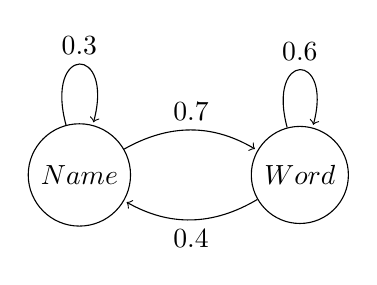
\begin{tikzpicture}[->,shorten >=1pt,auto,node distance=2.8cm]
  \tikzstyle{every state}=[]

  \node[state] (A)              {$ Name $};
  \node[state] (B) [right of=A] {$ Word $};

  \path (A) edge [loop above] node {0.3} (A)
            edge [bend left]  node {0.7} (B)
        (B) edge [bend left]  node {0.4} (A)
            edge [loop above] node {0.6} (B);
\end{tikzpicture}
\caption{Graph describing the transitions in a Markov Chain example.}
\label{fig:markov_graph}
\end{figure}

With the \textit{Time Invariance Assumption}, all parameters in our model can be described 
by a $ m \times m $ transition matrix $ \theta $ where each element $ \theta_{a, b} $ with
row $ a $ and column $ b $ holds the probability of going from state $ S_a $ to $ S_b $.
Naturally, the probabilities of row $ \theta_{a, *} $ must sum up to one since they represent
the entire scope of transition possibilities starting from state $ S_a $.
Equation \ref{eq:transition_matrix} describes a $ 2 \times 2 $ transition matrix 
$ Z $ for the same \textit{Markov Chain} example described in Figure~\ref{fig:markov_graph}.

\begin{equation}
Z = 
\begin{bmatrix}
    0.3 & 0.7 \\
    0.4 & 0.6 \\
\end{bmatrix}
\label{eq:transition_matrix}
\end{equation}

If we know the transition matrix $ \theta$ for a \textit{Markov Chain}, we can easily calculate 
the probabilities of being in each state at time $ t $. Consider that $ \rho_t $ is a vector of 
size $ m $ (i.e. the number of possible states) with the probabilities for each state
at time $ t $. Then:

\begin{equation}
\rho_{t+1} = \rho_t \cdot \theta
\end{equation}

And, for an arbitrary number of timesteps $ t \geq 0 $:

\begin{equation}
\rho_{t} = \rho_0 \cdot \theta^t
\end{equation}

Where $ \rho_0 $ is the vector of starting probabilities for each state. If we
know nothing about the initial conditions of our \textit{Markov Chain} we can simply 
assign the same probability to each state. 

The probability of observing a sequence of states $ X = \{ x_1, x_2, ..., x_n \} $
with an initial state $ x_0 $ is:

\begin{equation}
P(X) = P(x_0) \prod_{t=1}^{n} P(x_t|x_{t-1}) \\
\end{equation}

Now, to obtain the likelihood $ \mathcal{L(X; \theta)} $ we need only replace the
probabilities with the respective parameters in our model:

\begin{equation}
\mathcal{L}(X; \theta) = \rho_0 \prod_{t=1}^{n} \theta_{x_t, x_{t-1}}
\end{equation}

By defining $ \eta_{a,b} $ to be the count of transitions from $ a $ to $ b $ in 
$ X $. We can write the likelihood as:

\begin{equation}
\mathcal{L}(X; \theta) = \rho_0 \prod_{a, b} \theta_{a, b}^{\eta_{a, b}}
\label{eq:hmm_likelihood}
\end{equation}

Next we want to obtain the maximum likelihood estimator for the transition matrix $ \hat\theta $.
The likelihood function is always positive, so finding the set of parameters 
that maximizes the log likelihood $ \mathcal{l}(X; \theta) $ is equivalent to finding 
the parameters that maximize the likelihood itself. With the log likelihood, we transform the 
product over transition probabilities into a sum of logarithms, which is easier to work with.

\begin{equation}
\mathcal{l}(X; \theta) = log(\rho_0) \sum_{a, b} \eta_{a, b} \cdot log(\theta_{a, b})
\end{equation}

This way, we want to find $ \hat\theta $ such that:

\begin{equation}
\hat\theta = \argmax_{\theta} \mathcal{l}(X; \theta)
\end{equation}

However, if we try to optimize this function as it is, we will find that
$ \hat\theta_{a, b} = \infty, \forall a, b $. This happens because every row in 
the transition matrix  must sum up to one so the degrees of freedom for the model 
are actually $ m(m-1) $ and not $ m^2 $. This means that:

\begin{equation}
\sum_{b} \theta_{a, b} = 1, \forall a \in [1, m]
\end{equation}

A way to incorporate this constraint in our optimization problem is with the aid of
\textit{Lagrange Multipliers}. So we define the \textit{Lagrangian}:

\begin{equation}
Lag(\theta, \lambda) = \mathcal{l}(X; \theta) - \sum_{a} \lambda_{a} \cdot \left( \sum_{b} \theta_{a, b} - 1 \right)
\end{equation}

Taking the derivatives of $ Lag(\theta, \lambda) $ relative to $ \theta_{a, b} $ and making 
them equal to zero we get:

\begin{eqnarray}
\frac{\partial Lag(\theta, \lambda)}{\partial \theta_{a, b}} & = & \frac{\eta_{a, b}}{\theta_{a, b}} - \lambda_a = 0 \\
\theta_{a, b} & = & \frac{\eta_{a, b}}{\lambda_a} \\
\end{eqnarray}

And finally, by using the constrain equations $ \sum_b \theta_{a, b} = 1 $, we find that:

\begin{eqnarray}
\sum_b \frac{\eta_{a, b}}{\lambda_a} = 1 \\
\lambda_a = \sum_b \eta_{a, b} \\
\theta_{a, b} & = & \frac{\eta_{a, b}}{\sum_{b'} \eta_{a, b'}} \\
\end{eqnarray}

Yielding a closed form expression for the maximum likelihood estimator $ \hat\theta_{a, b} $.
What is really convenient, since this is the average number of transitions from state $ a $ to state
$ b $ in sequence $ X $. A value that can be easily obtained in $ O(n) $ time complexity. 

So far, we have assumed that all states $ X $ are observable, but in \textit{NER}, only the words 
are observed, while the \textit{Named Entity} labels associated with these words are not. That is why we need
another layer of complexity. The \textit{Hidden Markov Model (HMM)} differs from the \textit{Markov Chain} in that it 
does not observe the states $ X $ directly, but rather a probabilistic function of these states. 

With the \textit{Hidden Markov Model} we want to predict a sequence of labels $ Y = \{y_1, y_2, ..., y_n\} $ 
(i.e. the \textit{Markov Chain}) from a sequence of observed states $ X = \{x_1, x_2, ..., x_n\} $
(i.e. the words in a text). So we make an additional assumption:

\begin{equation}
P(x_i|y_{i-1}x_{i-1}, ..., y_1x_1) = P(x_i|y_i)
\end{equation}

That is, the probability of observing word $ x_i $ depends only on the current label
$ y_i $, the hidden state (e.g. PER, LOC, ORG, etc.). By making this assumption, we are
stating that if we know a token's assigned label, then we can reliably predict what are the 
probabilities that this token takes any value in a vocabulary. This is a very
simplistic assumption and many models (such as Conditional Random Fields) try to overcome this issue, 
but this step is necessary if we want to get a closed form estimator for our model. 
To model the emission probability distributions $ P(x_i|y_i) $, we assume again that 
the probabilities are time invariant and that $ x_i $ takes its value from a fixed vocabulary 
with size $ V $. Similar to the \textit{Transition Matrix}, we introduce a $ V \times K $ \textit{Emission Matrix} 
$ \mu $ where each cell $ \mu_{a,b} $ represents the probability that, 
given label $ a $, we will observe the word $ b $. 

Now, the probability of observing a vector of labels $ Y $ given a sequence of 
words $ X $ can be calculated with Bayes' theorem:

\begin{equation}
P(Y|X) = \frac{P(X|Y) P(Y)}{P(X)}
\end{equation}

Since $ P(X) $ is invariant for every sequence of labels $ Y $, we can simply 
optimize in terms of the joint probability $ P(X, Y) $:

\begin{equation}
P(Y|X) \propto P(X|Y) P(Y) = P(X, Y)
\end{equation}

And we get:

\begin{equation}
\mathcal{L}(Y|X; \theta) \propto \rho_0 
\prod_{a \in L, b \in L} \theta_{a, b}^{\eta_{a, b}} 
\prod_{c \in L, d \in V} \mu_{c, d}^{\eta_{c, d}}
\end{equation}

The parameters $ \theta $ and $ \mu $ are independent, so the procedure to find
$ \hat\theta $ remains the same. Also, we can employ the same procedure we used 
to find $ \hat\theta $ on \textit{Markov Chains} to find $ \hat\mu $ for
\textit{Hidden Markov Models}. This way we will find that:

\begin{equation}
\mu_{c, d} = \frac{\eta_{c, d}}{\sum_{d'}\eta_{d, c'}}
\end{equation}

This is the expected number of times we observed word $ d $ when we were at the state $ c $. A number
that is also easy to obtain in $ O(n) $ time. With that, we conclude the maximum likelihood parameter 
estimation for the \textit{Hidden Markov Model}. This procedure presupposes that we have labeled 
data, since we need to observe the correct labels $ Y $ to calculate $ \hat\theta $ and $ \hat\mu $. 
If we only have unlabeled data, we can do the parameter estimation with the Baum-Welch algorithm, 
though the results are much less reliable on the sequence labelling task. 

The last task we need to do is to calculate the most likely sequence of labels given a sequence of
observations. To obtain this sequence exactly we can employ the Viterbi algorithm, which is explained in Appendix
(REF). For higher order Hidden Markov Models the best sequence of labels can be computed 
with a variable state Viterbi approach \cite{Li2000}. However, as we increase $ k $, this computation 
becomes exponentially more expensive. The beam-search strategy may be employed for a faster 
search, but we found that for $ k \leq 4 $, the Viterbi algorithm is still viable.

(DISCUSS HOW TO SMOOTH WITH LAPLACE SMOOTHING)

(CITE MCCALLUM HERE)
HMM based taggers have been successfully applied in many NLP and WDE tasks 
\cite{Rabiner1990,Leek1997,Freitag2000}. They are incredibly fast to train and also they are very 
interpretable, making them a good choice for a first approximation. However, these models 
are highly dependent on the right selection of features, what may outweigh the benefit of a 
small training cost.

\subsection{Maximum Entropy Models and Linear Chain Conditional Random Fields}

(DISCUSS HOW UP TO THIS POINT WE HAVE BEEN WASTING MODELLING EFFORT ON MODELLING 
THE JOINT DISTRIBUTION AND WE COULD GO DIRECTLY TO THE CONDITIONAL)

An example of Maxent classifier for sequence tagging: https://www.aclweb.org/anthology/W96-0213.

% Good derivation of maxent classifier for NLP:
% http://www.ai.mit.edu/courses/6.891-nlp/READINGS/adwait.pdf
% https://repository.upenn.edu/cgi/viewcontent.cgi?article=1083&context=ircs_reports

A \textit{Linear Chain Conditional Random Field} is the particular case of a 
\textit{Conditional Random Field} where the labels are conditionally independent 
given the previous observations. (THIS SENTENCE HAS TO BE CHECKED). It is the
generalized case of a Maximum Entropy Markov Model, which is itself a combination of
Maximum Entropy Classifier for sequences.

The task of labeling sequences in \textit{Natural Language Processing} can be seen
as a classification task where we want to predict a label $ y $, given a word and its 
context, which we call jointly as $ x $. This context can be composed of any relevant 
features extracted from the text, such as surrounding words, previous labels, and sentence 
length. Because of its mathematical properties, the \textit{Maximum Entropy} framework provides 
a compelling way for estimating the probability of a label given its linguistic context, that is
$ P(Y|X) $.

The concept of Information Entropy established by Shannon (CITE HERE, A mathematical 
theory of communication) aims to quantify the
amount of information expressed in a statistical distribution. Namely, the entropy $ H $ of
a probability distribution X with a probability mass function $ p $ is given by:

(THE ENTROPY HERE SHOULD BE THE JOINT ENTROPY BETWEEN WORDS AND TAGS)

\begin{equation}
H(p) = \sum_{x \in X} p(x) \cdot log_2 \left( \frac{1}{p(x)} \right)
\end{equation}

In fact, the logarithm in the entropy function can be taken in any base. The change 
of base will only provide a linear scaling of the same entropy function. In this case,
$ H(p) $ is essentialy the expected number of bits necessary to encode the value of a
single random outcome drawn from $ X $, that is $ E[log_2 \left( \frac{1}{p(X)} \right)] $.
The more bits we need to encode the possible outcomes from a probability mass function, 
the more uncertain we are about the underlying distribution. For example, if an event has
only one possible outcome, we always know the value of a random sample, therefore
$ H(p) = 0 $ and the entropy is minimum. On the other end, if the probability distribution is
uniform, all outcomes have the same probability, and therefore we are as uncertain as we can be
and the entropy is maximum.

The principle of maximum entropy (CITE HERE) [Jaynes, 1957, Good, 1963]
states that, when we do not know exactly what probability 
distribution generated a sample, the best estimate for the parameters of this probability
distribution is the one that makes the least assumptions, or the one with maximum entropy. 
This is the distribution that is closest to the uniform distribution. 

A similar argument can be made to limit the number of free parameters in the model. That is,
when comparing two models with similar predictive power, the one with the least degrees of 
freedom should be prefered. However in practice, this is rarely taken into account.

The principle of maximum entropy is similar to a principle in the philosophy of science called Occam's Razor, 
that is, when there are two explanations for an outcome, the one that makes
the least number of assumptions is the best. Which is a good rule of thumb for science in general,
eventhough, ultimately nothing guarantees that the rules that explain reality will be simple.

Naturally, if we 
optimize the objective function without constraints, we will find that the \textit{Maximum Entropy} 
estimator will yield an uniform distribution, meaning that we are no better than simply predicting 
labels at random for our data. So, it becomes necessary to establish some constraints over
our optimization problem.

The choice of constraints is more or less arbitrary, but under the \textit{Maximum Entropy} 
framework, there is a strong motivation for setting these constraints in a way that makes
the \textit{Maximum Entropy} estimator equivalent to the \textit{Maximum Likelihood} estimator
for our model. By doing it, we can make sure that the model fits the data as tightly as possible
(the maximum likelihood estimate), while making as few assumptions as it needs to 
(the maximum entropy estimate). 

If we set these constraints such that, given $ k $ binary feature functions $ f_i $,
we have $ k $ constraints:

\begin{eqnarray}
E_{p(a,b)}[f_i] = \sum_{x} \tilde{p(a)} p(b|a) f_i(x) \\
E_{\tilde{p(a,b)}}[f_i] = \sum_{x} \tilde{p}(x) f_i(x) \\
E[f_i] = E_{\tilde{p(x)}}[f_i], \forall i \in \{ 1, 2, \dots, k \}
\label{eq:maxent_constraints}
\end{eqnarray}

On which $ E[f_i] $ is the model expectation of $ f_i $ and $ E[\hat{f_i}] $ is the 
observed expectation $ f_i $. And we maximize the conditional entropy subject to these
constraints:

\begin{equation}
H(p) = - \sum_{a, b} \tilde{p}(b) p(a|b) log p(a|b)
\end{equation}

Note that we use the simplification $ \tilde{p}(b) \approx p(b) $ suggested by 
Berger et. al., because the probability space of $ p(b) $ is too big to allow 
a simple calculation. (PAGE 12 of http://www.ai.mit.edu/courses/6.891-nlp/READINGS/adwait.pdf)

BERGER is here https://www.aclweb.org/anthology/J96-1002.

We can once again resort to Lagrange Multipliers to transform this problem into an
unconstrained optimization problem. The Lagrangian $ \Lambda $ takes the form:

\begin{equation}
\Lambda(p, \theta, \theta_p, \lambda, \beta) = H(p) 
+ \sum_{i}^n \lambda_i (E_{p(x)}[f_i] - E_{\tilde{p(x)}}[f_i]) 
+ \beta (\sum_{x,y} \tilde{p}(x) p(y|x)) - 1
\end{equation}

Now we need to make set all derivatives equal to zero to find the point that maximizes
the Lagrangian, and by consequence the conditional entropy subject to our constraints.
The derivatives relative to $ \lambda $ and $ \beta $ simply yield the initial constraints.
Now the the derivative relative to $ p $ is:

\begin{eqnarray}
\frac{\partial \Lambda}{\partial p} = -1 - log p(y|x) + \beta + \sum_i^n \lambda_i f_i(x, y) = 0 \\
p(y|x) = exp(\sum_{i}^n \lambda_i f_i(x, y) + \beta + 1)
\ref{eq:logistic_1}
\end{eqnarray}

Also, we know by our initial constraints that:

\begin{eqnarray}
\sum_y p(y|x) = 1 \\
\sum_y exp(\sum_{i}^n \lambda_i f_i(x, y) + \beta + 1) = 1 \\
e^\beta \cdot \sum_y exp(\sum_{i}^n \lambda_i f_i(x, y) + 1) = 1 \\
e^\beta = \frac{1}{\sum_y exp(\sum_{i}^n \lambda_i f_i(x, y) + 1)} \\
\end{eqnarray}

By replacing $ \beta $ in Equation~\ref{eq:logistic_1} we finally get:

\begin{equation}
p(y|x) = \frac{exp(\sum_{i}^n \lambda_i f_i(x, y))}{\sum_y exp(\sum_{i}^n \lambda_i f_i(x, y))}
\label{eq:logistic_1}
\end{equation}

At this point, we know that the model that maximizes the conditional entropy subject to the constraints
established in (REFERENCE TO CONSTRAINTS) has to belong to the parametric family described in 
Equation~\ref{eq:logistic}. This equation describes a family of exponential probability models known as 
logistic classifiers or maximum entropy classifiers, this is the unique solution to our optimization
problem (CHECK APPENDIX).

(SKETCH THE PROOF FOR UNICITY HERE)

Furthermore, by maximizing the Lagrangian $ \Lambda $ we can find the optimal set of 
parameters $ \lambda_i $ (a results granted by the Kuhn-Tucker theorem). This optimization
problem is identical to maximizing the log likelihood:

(THIS RESULT SHOULD BE BETTER EXPLORED)

\begin{equation}
\mathcal{L}(Y|X; \theta) = log \prod_{x, y} p(y|x)^{\tilde{p}(x,y)} = \sum_{x, y} \tilde{p}(x,y) log p(y|x)
\end{equation}

When the training samples are independent, maximizing the likelihood 

And this is essentialy the same thing as maximizing the cross-entropy 
(https://peterroelants.github.io/posts/cross-entropy-logistic/).
Now, there is no closed form expression to find the optimal set of parameters $ \theta $ 
that maximizes the likelihood / entropy, so we must resort to numerical optimization methods such 
as Stochastic Gradient Descent or L-BFGS. 

In the particular case of sequence labeling, the simplest conceivable classifier inside the Maximum Entropy
Framework would be a multinomial logistic regression that decodes each label independently. That is, given
a context $ x $ the classifier would predict a label $ y $ without taking in consideration any of the
previous or forward labels. This would be the discriminative analogue to the Naive Bayes model. However, 
the independence assumption is too restrictive for most language related tasks. Maximum Entropy
Markov Models (MEMM) try to overcome this problem by incorporating the insights obtained from Hidden Markov
Models into the Maximum Entropy Models while preserving the flexibility of discriminative models.


\begin{figure}[h]
  \centering
  \includegraphics[width=0.75\textwidth]{img/memm}
  \caption{HMM VS MEMM}
  \label{fig:memm}
\end{figure}

In MEMMs, we assume that the label probabilities are connected in a Markov Chain like in a HMM. However,
in HMMs we have transition probabilities $ P(Y_t|Y_{t-1}) $ and emission probabilities $ P(X_t|Y_t) $,
but in MEMMs we have a single transition function $ P(Y_t | Y_{t-1}, X_t) $ that combines evidence from
the previous state $ Y_{t-1} $ and the observations $ X_t $. Observe that, with this model we do not care
about the probability of the observations $ X_t $ in contrast to generative models, that model the joint
probability $ P(x, y) $. Because of this, the feature vector $ X_t $ may contain overlapping and 
non-independent features since there is no independence assumption. 

In MEMMs, we have $ |Y| $ transition functions $ P_{y'}(y|x) = P(y|y', x) $, each constituting a 
different model that has the exponential form:

\begin{equation}
P_{y_{t-1}}(y_t|x_t) = \frac{1}{Z(y_{t-1}, x_t)} exp(\sum_i(\lambda_i f_i(y_{t-1}, x_t)))
\end{equation}

Where $ Z(y', x) $ is a partition function that guarantees that the distribution over the next 
states $ s $ sums to one, starting from the previous state $ s' $. That is, each exponential
function is normalized locally in the context of the defining state $ s' $. Like the exponential
models described earlier, this form is a unique distribution that maximizes the entropy 
and the likelihood subject to the constraints that the expected value of each feature in the learned 
distribution agrees with the expected value in the training set, starting from state $ s' $.

We can calculate the probability for a sequence of labels by chaining the transition probabilities:

\begin{equation}
P(y*| x*) = \prod_{i=1} P_{y_{i}}(y_i|y_{i-1}, x_i)
\label{eq:sequence_memm}
\end{equation}

And the most probable sequence can be easily calculated with the Viterbi algorithm, as we did in HMMs.
Originally, the maximum entropy/likelihood parameters for the MEMM were calculated with Generalized
Iterative Scaling algorithm, but this method has fallen out of favor in face of gradient based 
numerical optimization methods such as SGD. 
It is also possible to perform parameter estimation with incomplete labels by employing a variation 
of the Baum-Welch algorithm.

MEMMs provide a more flexible approach to the problem of sequence labeling in comparison with 
HMMs, however they suffer from the label bias problem. To understand the label bias problem,
consider the case where we have a MEMM named entity classifier that aims to label person names
and locations in a sentence.

\begin{figure}
\centering
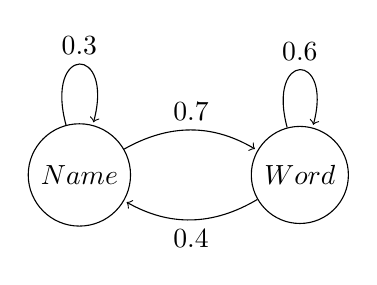
\begin{tikzpicture}[->,shorten >=1pt,auto,node distance=2.8cm]
  \tikzstyle{every state}=[]

  \node[state] (A)              {$ Name $};
  \node[state] (B) [right of=A] {$ Word $};

  \path (A) edge [loop above] node {0.3} (A)
            edge [bend left]  node {0.7} (B)
        (B) edge [bend left]  node {0.4} (A)
            edge [loop above] node {0.6} (B);
\end{tikzpicture}
\caption{Graph describing the label bias problem.}
\label{fig:markov_graph}
\end{figure}

INSERT HERE EXPLANATION OF LABEL BIAS PROBLEM FOR SEQUENCE LABELING

% 10 sentences in corpus where 9 times Summer Harris is a person and 1 time it is a location
% 10 sentences in corpus where 1 time  Summer Hall is a person and 9 times it is a location

Conditional Random Fields solve the label bias problem by jointly decoding the entire 
sequence of labels. That is, instead of normalizing the transition probabilities at each timestep as
described in Equation~\ref{eq:sequence_memm}, we normalize the probabilities for the entire
sequence of labels, that is:

\begin{eqnarray}
P(Y|X) = \frac{1}{Z(x)} \prod_{t=1}^{T} exp \left( \sum_{k=1}^{K} \theta_k f_k(y_{t-1}, y_t, X) \right) \\
Z(x) = \sum_{Y} \prod_{t=1}^{T} exp \left( \sum_{k=1}^{K} \theta_k f_k(y_{t-1}, y_t, x) \right)
\end{eqnarray}

The space of label combinations $ y' $ is huge $ |Y|^n $, being $ n $ the sequence length.

VERY GOOD TUTORIAL ON CRFs: https://homepages.inf.ed.ac.uk/csutton/publications/crftut-fnt.pdf

which is a sum over all possible label assignments $ Y $. The partition function can be efficiently
and exactly calculated with the sum-product algorithm. Parameter estimation is usually done through 
negative log likelihood minimization. The function can be optimized with techniques suitable for other 
maximum entropy models such as L-BFGS \cite{Liu1989}. The most likely label sequences can be decoded 
with the Viterbi algorithm, as was the case for HMMs.

CRFs are more general than HMMs because the transitions from $ y_{t-1} $ to $ y_{t} $ can depend 
on the whole vector of observations $ X $. This flexibility of feature functions allows for a wide range of
possibilities. 

Recently, Maximum Entropy Markov Models and Conditional Random Fields have been largely replaced
by neural network based models. However, Conditional Random Fields are still employed as the output 
layer of complex neural architectures.


\section{Neural Network Architectures}

The recent upsurge in the popularity of neural networks owes to the increasing computational 
capacity brought by Graphical Processing Units and discoveries such as Deep Belief Networks 
(CITE HINTON) in 2006 Autoencoders(?) and LSTMs (CITE HOCHREITER) in 1997 that helped overcome 
the limitations of earlier neural architectures. Deep neural architectures established new state 
of the art results for problems ranging from computer vision to speech recognition.

Neural networks are a family of classification algorithms that were vaguely inspired in the 
functioning of the human brain. They consist of a weighted graph of
artificial neurons, which are functions that receive an input from other neurons or from an input vector
and produce an output according to their activations. Neural networks are a general framework that can
encompass other machine learning approaches. For example, a single layer neural network with a softmax
activation function is equivalent to a multinomial logistic classifier (PUT PICTURE HERE)
Rosenblatt 1958). 

% D. R. Cox. 1958. The regression analysis of binary sequences. Journal of the Royal Statistical Society, Series B (Methodological), 20(2):215�242.

An extension of the logistic classifier to a neural network with multiple layers can still be trained 
the same way as the original model, that is, by minimizing the cross entropy. However, once we add multiple layers on top of
the logistic classifier, the optimization problem no longer retains its convexity. This means that 
numerical optimization methods can get trapped on local minima and miss the best set of parameters
for the model. For a long time, this limitation hindered the development of neural architectures. Nonetheless, 
in practice, the rugged shape of the cost function seems to be of minor 
importance. Even though the global optimization is not guaranteed, in most classification scenarios 
finding a local optimum solves the parameter estimation problem sufficiently well. Also, heuristic 
methods such as adding momentum to gradients can help the optimization algorithm avoid being trapped.

The topic of neural networks is incredibly vast and cannot be properly discussed in this
dissertation. For a thorough view of the field consult (CITE BENGIO DEEP ARCHITECTURES FOR AI).

In contrast to earlier probabilistic models that were more statistically oriented, many improvements 
to neural networks derive from empirical results obtained in specific applications. 
In the probabilistic modelling of text, we are especially interested in the subclass of recurrent 
neural networks (RNN).
RNNs have been successfully employed on numerous NLP tasks such as
language modelling, POS tagging, speech recognition and NER. In RNNs, some of the neuronal layer 
activations become inputs to the same layer at the next timestep. Additionaly,
different from feed-forward neural networks, RNNs can retain information in their internal state. 
This characteristic can function as a memory cell, preserving long distance relationships across the chain,
and making them more suitable for processing sequences, and consequently for solving text related tasks. 
Figure~\ref{fig:rnn_network} describes an RNN for sequence labeling unrolled through multiple 
timesteps. 

\begin{figure}[h]
  \centering
  \includegraphics[width=0.75\textwidth]{pics/rnn_network}
  \caption{RNN for NER}
  \label{fig:rnn_network}
\end{figure}

At each timestep, the neural network computes a hidden state $ h_t $ using an input 
vector $ x_t $ and the previous hidden 
state $ h_{t-1} $, that retains information from past 
iterations. The input vector $ x_t $ for our RNN can consist of word features similar to 
the ones used in the previously discussed statistical models encoded in one-hot vectors,
word embeddings or a combination of both.
Finally, the RNN produces an output vector $ y_t $ representing the label for that 
timestep. A common definition for an RNN cell is given by the equations:

\begin{flalign*}
h_t &= tanh(W_x x_t + W_h h_{t-1}) &\\
y_t &= softmax(W_y h_t) &
\end{flalign*}

Where $ W_x $, $ W_h $ and $ W_y $ are weight matrices that can be trained with the 
Backpropagation Through Time (BPTT) algorithm. On a sequence labeling task, $ W_y $ 
is a $ |H| \times |Y| $ weight matrix where $ H $ is the size of the hidden layer,
defined experimentally according to the task, and $ Y $ is the number of classification labels
for our problem. With the softmax activation, the RNN will generate a probability distribution
across the range of possible labels and we can simply select the most probable label at each
timestep, assuming independence between labels. Theoretically, RNNs are capable of learning
and retaining long term dependencies with their internal state $ h_t $. However, in practice,
it becomes difficult due to the vanishing gradient problem. 

(INSERT EXPLANATION OF VANISHING GRADIENT PROBLEM HERE)

Long short term memory networks (LSTM) were 
introduced by Hochreiter and Schmidhuber \cite{Hochreiter1997} with this problem in mind and 
have been popularized since then. 

LSTMs incorporate a memory cell $ c $ in the RNN definition and three gates to control 
the flow of information that comes in and out of the memory cell.
The input gate $ \Gamma_{i} $ controls the amount of new information that will flow into the memory cell,
the forget gate $ \Gamma_{f} $ controls the amount of previous information that will be retained in the memory
cell, and the output gate $ \Gamma_{o} $ controls the amount of information stored in the memory cell that
will be used to compute the output activation of the LSTM unit. 
LSTM cell implementations vary slightly in the literature. A visual description of 
our LSTM cell is provided in Figure~\ref{fig:lstm_cell}.

\begin{figure}[h]
  \centering
  \includegraphics[width=0.75\textwidth]{pics/lstm_cell}
  \caption{LSTM Cell}
  \label{fig:lstm_cell}
\end{figure}

The equations for the LSTM cell are:

\begin{flalign*}
\Gamma_{i} &= \sigma(W_i \cdot [x_t,h_{t-1}] + b_i) &\\
\Gamma_{f} &= \sigma(W_f \cdot [x_t,h_{t-1}] + b_f) &\\ 
\Gamma_{o} &= \sigma(W_o \cdot [x_{t},h_{t-1}] + b_o) &\\
c_t        &= \Gamma_{f} \ast c_{t-1} + \Gamma_{i} \ast tanh(W_c \cdot [x_{t},h_{t-1}] + b_c) &\\
h_t        &= \Gamma_{o} \ast tanh(c_t) &
\end{flalign*}

Where $ \sigma $ is the logistic sigmoid function. $ \Gamma_i $, $ \Gamma_f $, and $ \Gamma_o $ are the input,
forget and output gates, respectively, and $ W_i $, $ W_f $, $ W_o $ are the weight 
matrices corresponding to each gate. $ c_{t} $ is the cell 
state at time $ t $ and $ h_{t} $ is the hidden state at time $ t $. 
The vector $ [x_{t},h_{t-1}] $ is formed by concatenating the current input vector 
$ x_{t} $ and the hidden vector from a previous timestep $ h_{t-1} $. Finally,
$ A \ast B $ represents the element-wise multiplication of matrices $ A $ and $ B $
and $ A \cdot B $ represents the dot product of $ A $ and $ B $.

This implementation differs from the LSTM cell described in Huang et al. \cite{Huang2015}
in that the gates $ \Gamma_i $ and $ \Gamma_f $ do not receive inputs from the previous 
cell state $ c_{t-1} $ and the output gate $ \Gamma_{o} $ does not receive inputs from the current cell 
state $ c_{t} $. This variation produces little difference in terms of model accuracy on
the performed task, but it reduces model complexity.

\subsection{BI-LSTM-CRF}
\label{sssec:lstm_crf}

On named entity recognition tasks, both past and future words are important 
to attribute a label at time $ t $, however a regular LSTM network only takes 
past states into consideration. A bidirectional LSTM solves this problem by stacking 
two regular LSTMs, and feeding them with observations in opposite directions. The first LSTM 
receives forward states and the second LSTM receives backward states. The hidden states from both 
networks can then be concatenated at each timestep to produce output labels. With this 
architecture, LSTM cells may use information from past and future timesteps to decide 
the label at time $ t $.

Huang et al. \cite{Huang2015} proposed a bidirectional LSTM with a CRF layer (BI-LSTM-CRF) on 
the output to tackle the sequence tagging problem. The main benefit of adding a CRF layer 
in the neural sequence model is that the labels are jointly decoded for a whole sentence 
instead of being predicted individually. Another possibility would be to use a beam search
decoder to find an optimal sequence of labels. Predicted tags should be highly correlated 
in a named entity recognition task, so it is desirable to predict sequences conjointly.
The BI-LSTM-CRF is described in Figure~\ref{fig:bi_lstm_crf}.

\begin{figure}[h]
  \centering
  \includegraphics[width=0.75\textwidth]{pics/bi_lstm_crf}
  \caption{Bidirectional LSTM-CRF}
  \label{fig:bi_lstm_crf}
\end{figure}

This architecture achieved an F1 score of 90.10 on the English data from the CoNLL-2003 
NER shared task \cite{Sang2003}, in contrast to 85.17 for a bidirectional LSTM without 
a CRF layer. 
In our experiments, the LSTM-CRF architecture uses a bidirectional LSTM with 100 
hidden states, no peepholes and input and output dropout layers with a dropout
rate of 0.5. The dropout layers have proven to be very important to prevent overfitting 
and allow better generalization.

\subsection{CNN character representations}
\label{sssec:lstm_crf_cnn}

Ma and Hovy \cite{Ma2016} proposed to add a convolutional neural network (CNN) layer 
on top of a bidirectional LSTM-CRF to encode character-level information. The CNN
layer is described visually in Figure \ref{fig:cnn}.

\begin{figure}[h]
  \centering
	  \includegraphics[width=0.75\textwidth]{pics/cnn}
  \caption{CNN based character representations}
  \label{fig:cnn}
\end{figure}

The convolutional neural network receives character embeddings as inputs. The character 
representations generated by the CNN are combined with word level representations 
and fed to the BI-LSTM-CRF described in section \ref{sssec:lstm_crf}.
This architecture can learn morphological features that are very
useful in the NER task, since similar named entities often present morphological similarities. 
This architecture obtained an F1 score of 91.21 in the CoNLL2003 dataset. In our experiments, 
the LSTM-CRF architecture with CNN character representations uses a one dimensional convolutional 
neural network with 30 filters and a window size of three characters on top of the LSTM-CRF 
architecture. The character embeddings fed to the CNN have 30 dimensions that are randomly 
initialized.

\subsection{LSTM character representations}

Lample et al \cite{Lample2016} proposed to use a bidirectional LSTM to model character-level 
representations on top of a BI-LSTM-CRF. Combining the forward and backward LSTM hidden states 
to form the character representation, as described in Figure~\ref{fig:lstm_char}. 

\begin{figure}[h]
  \centering
  \includegraphics[width=0.75\textwidth]{pics/lstm_char_representations}
  \caption{LSTM based character representations}
  \label{fig:lstm_char}
\end{figure}

This character representation is also combined with a word 
representation and fed to a BI-LSTM-CRF network. 
The forward state is expected to be a better representation of the suffix of 
a token, and the backward state is expected to be a better representation of 
the prefix of a token. This differentiates the architecture
from the CNN based approach described in Section~\ref{sssec:lstm_crf_cnn}, because CNN filters 
discover positional invariant features, while LSTMs can better represent 
suffixes and prefixes. In our experiments, 
the LSTM-CRF architecture with LSTM character representations was implemented with a bidirectional 
LSTM with 25 hidden states, producing character representations of 
size 50. The character embeddings have 30 dimensions that are randomly initialized.

\subsection{Word Embeddings}

An important element of recurrent neural network architectures for text related tasks 
is the choice of word embeddings. Word embeddings are lower-dimensional representations of words in
continuous space. That is, each word is represented by a vector of continuous features (tipically a few hundred dimensions), 
often obtained with unsupervised clustering methods for words in large corpora. In comparison, one-hot encoded word 
vectors, that were popular before the introduction of word embeddings, are vectors with one dimension per 
word in the vocabulary (tipically a few hundred thousand dimensions) with 
zeros in all positions except for the index relative to that word. Figure~\ref{fig:word_embeddings} 
describes the difference between these two types of encodings. 

There are many advantages to the use of word embeddings relative to other encodings. First, 
the number of weights learned by the sequence model is smaller because of the dimensionality
reduction. Second, the mapping of words into feature vectors makes possible the comparison of similarity 
between words according to their shared features. Finally, and most importantly, word embeddings 
can be pretrained without supervision on large corpora and be used on tasks for which there is 
little labeled data. Pretrained word embeddings are a powerful form of transfer learning, what 
means bootstrapping the learning of model parameters by first training it on a bigger dataset. 
This is especially useful to the named entity recognition task, because named entitities that 
belong to the same class tend to have similar word embeddings. Thus, with good word embeddings, 
a neural network can predict the correct label for a word that was never seen in training
because of its similarity to other words that occurred in the training set.

Pretrained word embeddings can also be further improved by fine tuning the feature values in the 
specific problem of sequence labeling, by allowing backpropagation to alter the embeddings. However, 
due to the limited size of most sequence labeling datasets, this technique ends up introducing
noise to the word representations instead of improving the word representations.

There are multiple methods that produce word embeddings, and most of the official implementations 
also provide pretrained word embeddings for the English language. In this work, we explored
three sets of pretrained embeddings: Word2Vec, Glove and Elmo (CITE HERE). A brief description 
of these models is provided in Table~\ref{tab:word_embeddings}.

\begin{table}[h]
  \small
  \begin{center}
    \begin{tabular}{ ll }
      \toprule
      Model & Description \\
      \midrule
      Word2Vec & Regular HMM \\
      Glove    & HMM with $ k=2 $ \\
      Elmo     & HMM with $ k=3 $ \\
      \bottomrule
    \end{tabular}
  \end{center}
  \caption{Model descriptions}
  \label{tab:word_embeddings}
\end{table}

Most breakthroughs in sequence labeling tasks in the past few years came through the introduction
of novel methods for constructing word embeddings. Different from earlier methods such as Word2Vec and
Glove that produced static vectorial representations of words, more recent approaches such as
Elmo and Bert produce context dependent embeddings for a specific dataset with a neural network 
pretrained on a language modelling task. 


(HOW MUCH ELMO AND BERT HELPED IN THE CONLL-2003 TASK)

As word embedding and language modelling methods become more sophisticated, it comes to mind
if the complexity is justifiable. 
% https://d4mucfpksywv.cloudfront.net/better-language-models/language_models_are_unsupervised_multitask_learners.pdf
% https://openai.com/blog/better-language-models/

\subsection{Technical Concerns}

Eventhough word embeddings and character representations can make up for the feature engineering 
that was required by earlier statistical approaches to sequence labeling, there are still some
technical concerns to be faced that require quite a bit of engineering. The loss functions that need
to be optimized by our neural architectures is not convex, therefore the choice of the optimization 
function can impact the resulting set of parameters for our model as well as the parameter choice 
such as the learning rate for these functions. Neural networks are also prone
to overfitting, what can be partially avoided with the addition of dropout layers (CITE HERE)
or with the early stopping strategy over a validation dataset \cite{Caruana2000}. 

Another difficulty in training neural networks comes from the training time required for convergence
to a good set of parameters. This sometimes requires the employment of expensive hardware,
layer normalization https://arxiv.org/pdf/1607.06450.pdf and parallelization strategies. All of this
adds into the complexity, hardware cost and training cost of our models, many times providing only slight 
improvements over simpler approaches. This is not to say that simple models are preferable, but depending
on the task, deep neural architectures may be an over expensive approach.


\chapter{Sequence Labeling on HTML}

Up to this point, we have discussed sequence models that can be generally employed in 
many natural language tasks and also in other similar scenarios. However, there are
specificities related to the HTML structure and the problem of named entity  extraction 
on HTML that can be explored to allow further improvement at the researcher name extraction
task.

\section{Self training for Hidden Markov Models} 
\label{sec:self_training}

As described on Section~\ref{sec:hmm}. The simplest conceivable Hidden Markov Model 
for the sequence labeling on HTML task is a generative classifier that has the form:

\begin{equation}
P(X,Y) \propto \prod_{i=1}^n P(X_i|Y_i) P(Y_i, Y_{i-1})
\end{equation}

Where $ X $ is a sequence of words and $ Y $ is a sequence of labels, each with size $ n $.
This means we need to estimate the probabilities:

\begin{itemize}
  \item $ P(X_i|Y_i) $: the emission probabilities of word $ X_i $ given label $ Y_i $
  \item $ P(Y_i|Y_{i-1}) $: the transition probabilities of goind from label $ Y_{i-1} $ to label $ Y_i $
\end{itemize}

Surely, we may consider $ X_i $ to be a feature vector $ X_i = \{ f_{i,1}, f_{i,2}, ..., f_{i,k} \} $
as long as all the features are independent. That is:

\begin{equation}
P(X_i|Y_i) = P(f_{i,1}, f_{i,2}, ..., f_{i,k}|Y_i) = \prod_{j=1}^k P(f_j|Y_i)
\end{equation}

With this assumption, we can estimate parameters as described by the equations in Section~\ref{sec:hmm} 
(CITE SPECIFIC EQUATIONS). This approach yields consistent results, but if we try to use HTML features
such as the HTML element encompassing a word or the CSS classes related to this element, we will find
a problem. There is not much statistical similarity between the HTML structure in different web pages.
What this means is that, only because a given named entity label occurs more often inside "<div>" tags
in a page, that does not mean it is the case for most web pages. Consider for example a faculty web page 
that shows researcher names in a table ("<td>" tags) in contrast to a web page that organizes researcher
names in a list ("<li>" tags). If the first page is in our training set, the second page is in our test
set and we use the HTML tag feature to predict the labels of researcher names we will probably get many
wrong predictions.

Nonetheless, the HTML features are not useless. Inside a single web page, the HTML tag is a good predictor
for the label attributed to a word. A word's HTML context is a good predictor of its label. The question
is how to incorporate this intution in the Hidden Markov Model.

Consider a set of textual features unrelated to the HTML structure $ F^T = \{ f^T_1, f^T_2, ..., f^T_m \} $
a set of HTML features that are related to the HTML structure $ F^H = \{ f^H_1, f^H_2, ..., f^H_k \} $.
Next, consider two HMMs $ \phi_1 $ and $ \phi_2 $, where $ \phi_1 $ incorporates only the textual
features $ F^T $, while $ \phi_2 $ incorporates the whole set of features $ F^T \cup F^H $. Then,
if $ \tilde{\phi_1} $ is the Hidden Markov Model with maximum likelihood parameters for a given training 
set, we can estimate labels $ \tilde{Y} $ for the test set and approximate the probabilities 
$ P(f^H_{i}|Y) $ by:

\begin{equation}
P(f^H_{i}|y) \approx MLE_{\tilde{y}} P(f^H_{i}|y)
\end{equation}

Where $ MLE_{\tilde{y}} P(f^H_{i}|y) $ is the maximum likelihood estimator $ P(f^H_{i}|y $ considering 
that the predicted labels for our test $ \tilde{y} $ set are the correct labels. This self training
strategy can be implemented like this:

\begin{itemize}
\item Train the HMM without any HTML features.
\item Compute labels for a website with the trained HMM.
\item Use the computed labels as a proxy for the actual labels in the 
website and estimate HTML feature frequencies for this website alone.
\item Recompute the labels now using the HTML feature probabilities.
\end{itemize}

With some effort, this strategy could be incorporated in the Baum-Welch algorithm, but this heuristic
approach already yields a consistent improvement. In theory, this strategy could be used with any 
sequence tagger, however retraining a classifier with new features can become prohibitively expensive
depending on the algorithm being used. This strategy is only possible because the computation of HTML 
feature frequencies can be performed very quickly. This adds very little overhead to the original HMM 
and incorporates our intuition that HTML features are useful in sequence labeling tasks for HTML.

\section{Attentions Models} 

The self-training strategy for HMMs demonstrates a way to incorporate HTML features in 
sequence models, however it is not clear how to apply the same intuition to neural 
networks. Ultimately, we want the model to consider the predictions that it made for 
words in similar HTML contexts when constructing the neural representation for the 
current word in a sequence. A natural way to incorporate this intuition into the neural 
architectures described in Chapter~\ref{cha:neural_networks} is with the use of 
self attention mechanisms (https://papers.nips.cc/paper/7181-attention-is-all-you-need.pdf).
Originally, attention mechanisms were developed with the goal of solving sentence alignement 
for neural machine translation (https://arxiv.org/pdf/1409.0473.pdf), but since then it
found other uses in Natural Language Processing. An attention mechanism is a way to combine
inputs from multiple timesteps in a sequence to perform an operation at the current timestep.
Figure~\ref{fig:attention} describes an attention mechanism that incorporates evidence from
the whole sequence at time $ t $.

In a LSTM-CRF model, the bidirectional LSTM layer produces output representations at each 
timestep, producing a $ T \times H $ matrix $ \phi $, where $ T $ is the number of timesteps in the
sequence and $ H $ is the LSTM hidden layer size, which is defined arbitrarily (we omit
the batch size in this matrix representation). If the sequence length in the dataset varies,
we can simply pad the short sentences with zero vectors. In other words, the matrix $ \phi $ 
constitutes a neural representation for a sentence with vectors of size $ H $ representing
words at each timestep. In the original LSTM-CRF model without an attention layer, these
neural representations would be passed directly as features to a linear chain conditional random
fields decoder, but in the Self-Attended LSTM-CRF we add an attention mechanism between the LSTM
output and the CRF input as described in Figure~\ref{fig:lstm_attention}.

Now we need to find a way to combine the vectors at each timestep in a way that transforms 
the representations according to the similarity between HTML contexts. Essentialy, we want to compute a $ T \times T $ 
attention matrix $ alpha $ where $ alpha_{i, j} $ is the weight attributed to the word representation $ h_j $ at timestep
$ i $. In other words, $ alpha_t $ is measuring the amount of attention that we pay to all the words in 
a sentence at timestep $ t $. With the $ \alpha $ matrix, we can calculate new representations $ h'_i $ 
for each timestep by performing a linear combination of the hidden states according to their 
attention values:

\begin{equation}
h'_i = \sum_{j} = \alpha_{i, j} h_j
\end{equation}

Also, consider a set of $ n $ context vectors $ c_i $ that contain representations for the
html features at timestep $ i $. This representation can be a binary feature vector,
a dense vector or even the hidden states $ h_i $. The attention matrix is then calculated by:

\begin{equation}
\alpha_{i,j} = \frac{exp(A(c_i, c_j))}{\sum_k exp(A(c_i, c_k))}
\end{equation}

Where $ A(c_i, c_j) $ is an attention function that computes the similarity between
HTML contexts at timesteps $ i $ and $ j $ and outputs a real number. The exponentials are
a softmax normalization function to ensure that $ 1 \geq \alpha_{i,j} \geq 0 $ and 
$ \sum_{j} \alpha_{i, j} = 1 $. Now we propose two ways for defining the attention function
$ A $. The hard attention function and the soft attention function. The overall architecture 
for the attention mechanism in sequence labeling for HTML is described in 
Figure~\ref{fig:attention_for_html}.

\subsection{Hard Attention}

The hard attention function is a binary similarity function that either outputs one when 
contexts are identical or zero when they are different. This definition only makes sense
when the contexts $ c_i $ at timestep $ i $ are discrete feature vectors, because otherwise 
we would need a softer comparability criterion. So, if $ c_i = \{ f_{i,1}, f_{i,2}, ..., f_{i,m} \} $
is a context vector where each feature $ f_{i,j} $ assumes a definite value from a discrete set
$ \gamma_j $, we can define the attention function:

\begin{equation}
  A(c_i, c_j) = \begin{cases} 
    1 \text{ if } f_{i,k} = f_{j,k} \forall k \in m \\ 
    0 \text{ otherwise}
  \end{cases}
\end{equation}

The combination of features must be sufficiently restrictive so that the mixture of hidden
states does not introduce too much noise. We have determined experimentally that considering
only three features: the enclosing HTML tag, its parent tag and the CSS class; is sufficient to 
permit a consistent comparison between similar HTML contexts. Ideally, the choice of features
could be performed automatically with the incorporation of a feed forward neural network in
the comparison function and a softer similarity criterion. A possibility for doing this is 
presented in the Soft Attention function.


\subsection{Soft Attention}

Different from the hard attention function, the soft attention function outputs a real number 
that represents the degree of similarity between HTML contexts. Now, instead of considering
discrete feature vectors we resort to dense vectorial representations for the HTML context.
Similar to the way we extracted morphological features with characters representations in 
(CITE HERE lstm-crf-cnn and lstm-crf-lstm), we can extract HTML structural features with
DOM representations. To do this, consider a DOM tree (which is a directed graph),
a word's HTML context can be represented by the path we take in this graph starting from the 
root element as described in Figure~\ref{fig:html_graph}. If we consider the path for each
word in our sequence, we can create HTML dense representations by training a matrix of fixed
size embeddings for each HTML tag, then we can construct representations for these HTML 
embeddings the same way we did with character embeddings. The possibility that we chose 
is represented in Figure~\ref{fig:html_embeddings}. Since the vocabulary of HTML tags is 
very reduced, there is no need to pretrain the embeddings in a larger corpus.

Now to measure the similarity between different HTML contexts, we resort to an attention
function similar to the scaled dot product proposed by (CITE Attention is all you need). 
That is:

\begin{equation}
  A(c_i, c_j) = \frac{W c_i \cdot W c_j}{\sqrt{n}}
\end{equation}

Where $ W $ is a weight matrix to be learned and $ \sqrt{n} $ is a normalization factor
with $ n $ being the size of the contexts vectors $ c $. This function assumes a larger
value when the contexts are similar and a smaller value otherwise. With the soft attention
mechanism, our model can learn HTML context representations from the training data and
generalize intuition such as: if some words happen together in a list then they probably 
belong to the same class.


\subsection{Dataset split and Experimental Considerations}

In sequence labeling tasks, it is common to split the dataset in sentences and then train them
in independent steps. However, if we want to make use of attention mechanisms to 
perform the comparison of words in different HTML contexts, we want to compare the classes attributed 
to words in different sentences that share a similar context. That is why splitting the dataset
into sentences makes these mechanisms useless. To permit the comparison of words in different 
sentences, we combined multiple sentences in a single training step and separated them with a
segmentation token.

Also, the attention matrix calculations can become incredibly burdensome when we consider large
sentences or combinations of sentences. So, it becomes necessary to perform the matrix calculations
in a Graphical Processing Unit. And with the addition of many more parameters to the model, the 
risk of overfitting the training data becomes more salient. To prevent this problem from ocurring 
it is of utmost importance to add dropout layers before and after the attention mechanism.

\section{F1 Optimization} 

Normally, we want to estimate model parameters by maximizing the likelihood or minimizing the
cross entropy, which is equivalent when considering a softmax output layer. The likelihood is
intimately associated with the accuracy of a model, but in information extraction tasks we 
usually evaluate the performance of different models with other measures such as Precision, 
Recall and the F-measure. For example, in the Named Entity Recognition task many times we can 
get an accuracy that surpasses 90\% by simply labeling all tokens with an O (other) label, which
is the most common label. However, the F-measure for such a model would be zero. 

By maximizing the likelihood, we are essentialy increasing acccuracy with the expectation that this 
will lead to an improvement of the F-measure, what is true. However, since we ultimately want to 
maximize the F-measure, we could instead maximize an utility function that takes this into consideration. 
Also, the choice of F-measure for most problem is usually the F1-score, but depending on the
task, we may prefer more precision rather or more recall. Since usually there is a trade-off
inherent to the maximization of both measures, it would be useful if we had an utility function that
could take into consideration the particular precision and recall needs of a specific task.
In the case of named entity extraction on HTML, we could argue that recall is slightly more
important than precision, because when parsing a huge amount of data it is much easier to manually 
filter false positives from the results than manually finding false negatives that were missed by 
the classifier.

Nevertheless:

"while the F-measure of a classifier evaluated on a single supervised instance is well defined, the
overall F-measure on a larger dataset is not a function of the F-measure evaluated on each instance
in the dataset. This is in contrast to ordinary loss/utility, whose grand total (or average) on a dataset
can be computed by direct summation"

% http://www.cs.columbia.edu/nlp/papers/2005/jansche_05b.pdf

This makes the usage of the F-score as a utility function impractical for large datasets trained in 
batches. However, with a few simplifications we can replace our loss function and instead 
maximize the F-measure in terms of the expected utility. We take the method proposed by Jasche (CITE) to 
approximately maximize the F-measure of a classifier based on a logistical regression model and 
apply it to our neural architectures. The F-measure function can be calculated in terms of a triple (A,B,C):

\begin{equation}
F_\alpha(A, B, C) = \frac{A}{A + \alpha B + (1-\alpha) C}
\end{equation}

This is equivalent to the $ \alpha $-weighted harmonic mean defined in (CITE FSCORE FORMULA HERE).
A is the number of true positives, B is the number of false negatives, and C is the number of false
positives. Also, consider that:

\begin{eqnarray}
n_{pos} = A + B \\
m_{pos} = A + C
\end{eqnarray}

That is, $ n_{pos} $ is the number of positive examples in the dataset (true positives plus missed positives) 
and $ m_{pos} $ is the number of positive examples that were predicted (true positives plus false positives).
With this, we can rewrite $ F_\alpha(A, B, C) $ as:

\begin{equation}
F_\alpha(A, B, C) = \frac{A}{\alpha n_pos + (1-\alpha) m_pos}
\end{equation}

Now, Jasche propose the optimization objective:

\begin{equation}
\tilde{F}_\alpha(\hat{y}, y) = 
  \frac{\tilde{A}(\hat{y}, y)}
  {\alpha \tilde{n}_{pos} + (1-\alpha) \tilde{m}_{pos}(\theta)}
\end{equation}

For simplicity sake, we consider that we are dealing with a binary classification problem
with \textit{False} and \textit{True} labels. Then, $ \hat{y_i} $ is the label 
prediction made by our classifier for example $ i $ and $ \theta_i $ is the probability
that example $ i $ should take a \textit{True} label. Then, considering $ n $ examples:

\begin{eqnarray}
\tilde{A}(y, \hat{y}) = \sum_{i=1}^n I_{y = \hat{y} = 1} \cdot \theta_i  \\
\tilde{m}_{pos} = \sum_{i=1}^n \theta_i \\
\tilde{n}_{pos} = \sum_{i=1}^n I_{y=1} - \tilde{A}(y, \hat{y}) \\
\end{eqnarray}

With that, we have defined an optimization function that can be optimized with standard numerical optimization methods.
Different from the actual F-measure employed on a sequence labeling problem, we consider that each label here 
is independent and belongs to a different entity. Further work is needed to resolve this simplification and to 
adapt this optimization function to multi-label classification tasks.


\chapter{Experiments}

In our experiments, we wanted to determine the best sequence labeling methods for HTML by testing
their performance on a named entity recognition task over the NER on HTML dataset introduced in
Chapter~\ref{cha:ner_on_html}. Model performance was evaluated in terms of their accuracy, precision,
recall, F-score and overall simplicity, because some metric improvements require a significant 
amount of added complexity and training time.


\section{Simple Baseline}

Since the NER on HTML dataset is novel, we wanted to establish some baseline results in addition to
the gazetteer matching results presented in Table~\ref{tab:gazetter_matching}. For this purpose, we
trained a simple generative model and a simple discriminative model to provide a measure of the
expected difficulty for solving this task. The simple generative model is a Naive Bayes classifier,
which is essentialy a \textit{Hidden Markov Model}, as presented in Section~\ref{sec:hmm}, with the
assumption of label independence. That is, $ P(Y_i|Y_{i-1}) = P(Y_i) $ for timestep $ i $. The simple
discriminative model is a Logistic Classifier, as presented in Section~\ref{sec:max_ent}. 

The Naive-Bayes and Logistic classifiers form a generative-discriminative pair (CITE PAPER),
% http://ai.stanford.edu/~ang/papers/nips01-discriminativegenerative.pdf
in the sense that the essential difference between the models is that the first estimates the
joint probability between words and labels $ P(X, Y) $ and the latter models the conditional
probability $ P(Y|X) $. They are very simple and fast to train, so they provide a good 
first approximation to a solution for this task. We also consider model variants that incorporate
all the features presented in Table~\ref{tab:features} and variants that use no features beside
the current word. Table~\ref{tab:nb_and_maxent} shows a comparison between these models.

\begin{table}[h]
  \small
  \begin{center}
    \begin{tabular}{ lllllll }
      \toprule
      \multirow{2}{*}{Model} & \multicolumn{3}{c}{Validation} & \multicolumn{3}{c}{Test} \\
                             & \multicolumn{1}{c}{P} & \multicolumn{1}{c}{R} & \multicolumn{1}{c}{F1}
                             & \multicolumn{1}{c}{P} & \multicolumn{1}{c}{R} & \multicolumn{1}{c}{F1} \\
      \midrule
      Gazetteer Matching     & 0.847 & 0.285 & 0.427 & 0.871 & 0.328 & 0.477          \\
      Naive Bayes            & 0.172 & 0.851 & 0.287 & 0.181 & 0.776 & 0.294          \\
      Maxent                 & 0.287 & 0.547 & 0.377 & 0.335 & 0.508 & 0.404          \\
      Naive Bayes + Features & 0.354 & 0.784 & 0.488 & 0.414 & 0.767 & \textbf{0.537} \\
      Maxent + Features      & 0.309 & 0.544 & 0.394 & 0.416 & 0.618 & 0.497          \\
      \bottomrule
    \end{tabular}
  \end{center}
  \caption{Naive Bayes and Logistic Regression performance}
  \label{tab:nb_and_maxent}
\end{table}

As previously discussed, the Maximum Entropy classifier allows for overlapping features while
Naive Bayes assumes feature independence. 
The maximum entropy classifier fares better when no features besides the current word are considered. 
Nevertheless, when considering 
the whole set of features, there is not much difference between the discriminative and generative 
approaches. So we consider the best F1-score in the test set (\textit{Naive Bayes} with features) as 
a baseline to compare how much better we can get as we increase the model complexity.


\section{Hidden Markov Models}

There are a couple of parameters that need to be considered when we employ \textit{Hidden Markov Models}
to a sequence labeling task. First, the number of previous states (the order of the HMM) and, second, 
the model features. 

\subsection{HMM order}

Table~\ref{fig:hmm_no_features} shows performance of \textit{HMMs} up to the third 
order in the validation and test sets of the NER on HTML dataset. We can see that considering label
dependencies over multiple timesteps increases the classifier performance by a considerable margin 
relative to the \textit{Naive Bayes} model even without the addition of any features. That is, the 
second order \textit{HMM} (HMM-2) achieved an F1-score of 0.583 at the task, while
the \textit{Naive Bayes} classifier that incorporated all features achieved only 0.537 F1-score. Nevertheless,
we already observe a relaive decline in performance with the third order \textit{HMM} (0.506 F1-score), 
suggesting that increasing the order of the \textit{HMM} is not always advantegeous.

\begin{figure}[h!]
  \begin{center}
    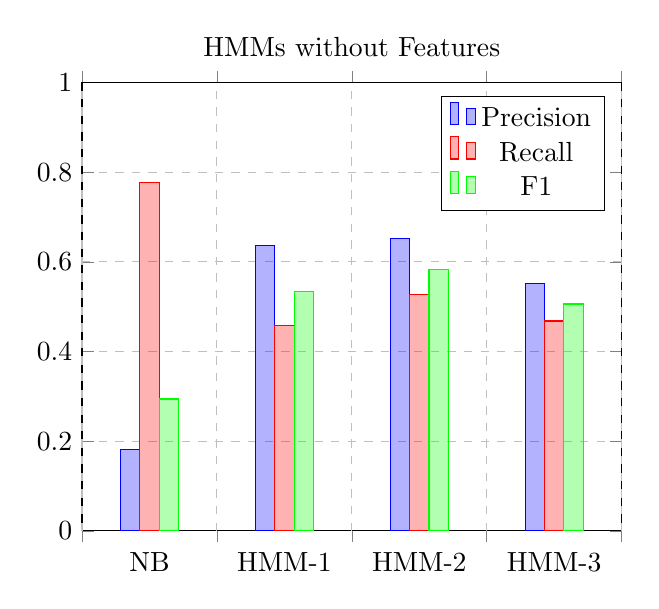
\begin{tikzpicture}
      \begin{axis}[
        title={HMMs without Features},
        xmin=0.5, xmax=4.5,
        ymin=0, ymax=1,
        xticklabels={NB,HMM-1,HMM-2,HMM-3},
        xtick={1,...,4},
        ytick={0,0.2,...,1},
        ybar=0pt,
        bar width=7pt,
        xtick distance=1,
        xtick style={
            /pgfplots/major tick length=0pt,
        },
        extra x ticks={-0.5,0.5,...,5.5},
        extra x tick labels=\empty,
        extra x tick style={
            grid=major,
            xtick style={
                /pgfplots/major tick length=4pt,
            },
        },
        ymajorgrids=true,
        grid style=dashed,
        legend pos=north east,
      ]

      \addplot[ybar, color=blue, fill=blue, fill opacity=0.3,] coordinates {
        (1,0.181)(2,0.637)(3,0.653)(4,0.551)
      };
      \addplot[ybar, color=red, fill=red, fill opacity=0.3,] coordinates {
        (1,0.776)(2,0.458)(3,0.527)(4,0.468)
      };
      \addplot[ybar, color=green, fill=green, fill opacity=0.3,] coordinates {
        (1,0.294)(2,0.533)(3,0.583)(4,0.506)
      };
      \legend{Precision, Recall, F1};
       
      \end{axis}
    \end{tikzpicture}
    \caption{
      Performance of the Naive Bayes classifier and Hidden Markov Models without 
      features besides the current word on the test set of the NER on HTML dataset.
    }
    \label{fig:hmm_no_features}
  \end{center}
\end{figure}

\subsection{Feature selection}

In the previous section, we considered a \textit{Naive Bayes} classifier that incorporated all the
features regardless of their correlations, eventhough we know that correlated features may 
hurt the performance of such a classifier. Table~\ref{tab:feature_correlation} presents a feature 
correlation matrix based on the Cram�r's V measure~\footnote{
Dpython implementation
% https://en.wikipedia.org/wiki/Cram%C3%A9r%27s_V
% https://github.com/shakedzy/dython/blob/master/dython/nominal.py
}. 

\begin{table}[h]
  \tiny
  \begin{center}
    \begin{tabular}{ lccccccccccc }
      \toprule
           & \rot{Word} & \rot{Exact Match} & \rot{Partial Match} & \rot{Email} & \rot{Number} & \rot{Honorific} 
	   & \rot{URL} & \rot{Capitalized} & \rot{Punctuation} & \rot{HTML Tag} & \rot{CSS Class} \\
      \midrule
      Word          & 1.00 & \textbf{0.60} & \textbf{0.94} & \textbf{1.00} & \textbf{1.00}  & \textbf{1.00} & 0.00 & \textbf{0.84} & \textbf{1.00}  & 0.25 & 0.00 \\
      Exact Match   & -    & 1.00  & 0.19  & -0.02 & -0.07 & -0.04 & 0.00 & 0.15  & -0.05 & 0.07 & 0.22 \\
      Partial Match & -    & -     & 1.00  & -0.11 & -0.35 & -0.09 & 0.00 & -0.01 & 0.45  & 0.04 & 0.17 \\
      Email         & -    & -     & -     & 1.00  & -0.02 & -0.02 & 0.00 & -0.12 & -0.05 & 0.03 & 0.27 \\
      Number        & -    & -     & -     & -     & 1.00  & -0.07 & 0.00 & -0.36 & -0.16 & 0.09 & 0.34 \\
      Honorific     & -    & -     & -     & -     & -     & 1.00  & 0.00 & 0.15  & -0.08 & 0.02 & 0.11 \\
      URL           & -    & -     & -     & -     & -     & -     & 1.00 & 0.00  & 0.00  & 0.00 & 0.00 \\
      Capitalized   & -    & -     & -     & -     & -     & -     & -    & 1.00  & -0.48 & 0.07 & 0.28 \\
      Punctuation   & -    & -     & -     & -     & -     & -     & -    & -     & 1.00  & 0.04 & 0.11 \\
      HTML Tag      & -    & -     & -     & -     & -     & -     & -    & -     & -     & 1.00 & \textbf{0.64} \\
      CSS Class     & -    & -     & -     & -     & -     & -     & -    & -     & -     & -    & 1.00 \\
      \bottomrule
    \end{tabular}
  \end{center}
  \caption{Feature correlation matrix}
  \label{tab:feature_correlation}
\end{table}

The current word is strongly correlated with most features besides the URL feature, and the ones related to 
the HTML structure. That shows there is not a lot of information gain from these features. To understand how
this can help or hurt the \textit{Hidden Markov Model} performance we test the model using two groups 
of features:

\begin{description}
  \item[Group A] Current word, Exact Match, Partial Match, URL, Capitalized
  \item[Group B] All features except HTML Tag and CSS Class
\end{description}

Table~\ref{tab:hmm_features} compares the performance of \textit{Hidden Markov Models} using the features from
Group A and Group B. The Group A model performed better in all criteria showing that the selection of features
is of the utmost importance for the application of \textit{HMMs} to the sequence labeling problem.

\begin{figure}[h!]
  \begin{center}
    \tiny
    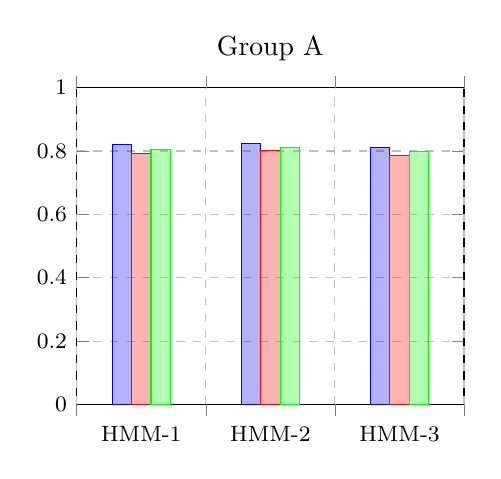
\begin{tikzpicture}
      \pgfplotsset{small}
      \begin{axis}[
        title={Group A},
        xmin=0.5, xmax=3.5,
        ymin=0, ymax=1,
        xticklabels={HMM-1,HMM-2,HMM-3},
        xtick={1,...,3},
        ytick={0,0.2,...,1},
        ybar=0pt,
        bar width=7pt,
        xtick distance=1,
        xtick style={
            /pgfplots/major tick length=0pt,
        },
        extra x ticks={-0.5,0.5,...,5.5},
        extra x tick labels=\empty,
        extra x tick style={
            grid=major,
            xtick style={
                /pgfplots/major tick length=4pt,
            },
        },
        ymajorgrids=true,
        grid style=dashed,
      ]

      \addplot[ybar, color=blue, fill=blue, fill opacity=0.3,] coordinates {
        (1,0.819)(2,0.823)(3,0.812)
      };
      \addplot[ybar, color=red, fill=red, fill opacity=0.3,] coordinates {
        (1,0.792)(2,0.802)(3,0.785)
      };
      \addplot[ybar, color=green, fill=green, fill opacity=0.3,] coordinates {
        (1,0.805)(2,0.812)(3,0.798)
      };
      \legend{};
       
      \end{axis}
    \end{tikzpicture}
    ~
    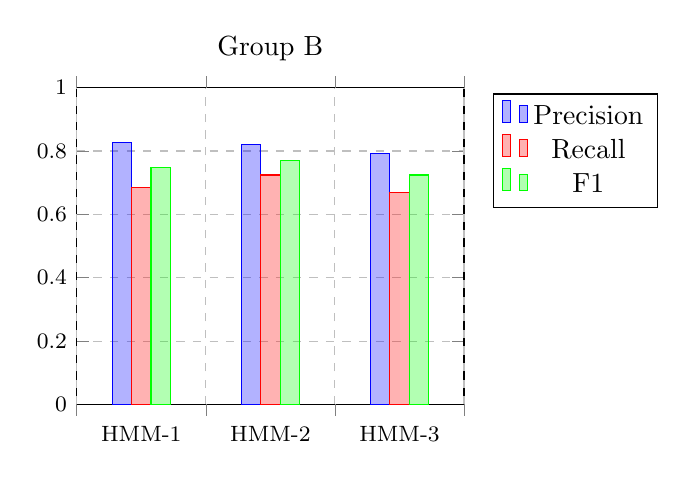
\begin{tikzpicture}
      \pgfplotsset{small}
      \begin{axis}[
        title={Group B},
        xmin=0.5, xmax=3.5,
        ymin=0, ymax=1,
        xticklabels={HMM-1,HMM-2,HMM-3},
        xtick={1,...,3},
        ytick={0,0.2,...,1},
        ybar=0pt,
        bar width=7pt,
        xtick distance=1,
        xtick style={
            /pgfplots/major tick length=0pt,
        },
        extra x ticks={-0.5,0.5,...,5.5},
        extra x tick labels=\empty,
        extra x tick style={
            grid=major,
            xtick style={
                /pgfplots/major tick length=4pt,
            },
        },
        ymajorgrids=true,
        grid style=dashed,
        % legend pos=north east,
	legend style={at={(1.5,0.8)},anchor=east},
      ]

      \addplot[ybar, color=blue, fill=blue, fill opacity=0.3,] coordinates {
        (1,0.826)(2,0.820)(3,0.791)
      };
      \addplot[ybar, color=red, fill=red, fill opacity=0.3,] coordinates {
        (1,0.684)(2,0.724)(3,0.668)
      };
      \addplot[ybar, color=green, fill=green, fill opacity=0.3,] coordinates {
        (1,0.748)(2,0.769)(3,0.724)
      };
      \legend{Precision, Recall, F1};
       
      \end{axis}
    \end{tikzpicture}

    \caption{Hidden Markov Models trained with the features in Group A and Group B.}
    \label{fig:hmm_all_features}
  \end{center}
\end{figure}

\subsection{Self-training strategy}

In the next experiment, we want to understand if the self-training strategy from 
Section~\ref{sec:self_training} is effective for improving the performance of 
\textit{HMMs}. Figure~\ref{fig:hmm_self_training} compares the performance of \textit{HMMs}
up to third order with features from \textit{Group A} and with the self-training 
strategy for the \textit{HTML Tag} and the \textit{CSS Class} features in addition to the 
\textit{Group A} features. The self-trained models show a marked improvement in comparison
to the models with no self-training at the test set except for the third order \textit{HMM}.
With this, we conclude that the best \textit{HMM} for the name extraction task is a 
second-order \textit{HMM} using \textit{Group A} features and the self-training strategy. This
model achieves an \textit{F1} of 0.879. The detailed results for all HMMs is presented in
Table~\ref{tab:hmm_results}.

\begin{figure}[h!]
  \begin{center}
    \tiny
    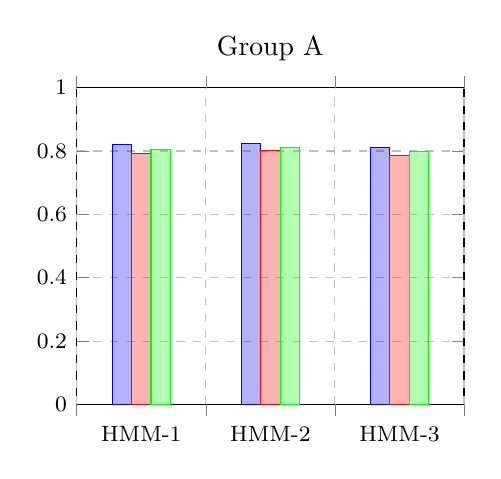
\begin{tikzpicture}
      \pgfplotsset{small}
      \begin{axis}[
        title={Group A},
        xmin=0.5, xmax=3.5,
        ymin=0, ymax=1,
        xticklabels={HMM-1,HMM-2,HMM-3},
        xtick={1,...,3},
        ytick={0,0.2,...,1},
        ybar=0pt,
        bar width=7pt,
        xtick distance=1,
        xtick style={
            /pgfplots/major tick length=0pt,
        },
        extra x ticks={-0.5,0.5,...,5.5},
        extra x tick labels=\empty,
        extra x tick style={
            grid=major,
            xtick style={
                /pgfplots/major tick length=4pt,
            },
        },
        ymajorgrids=true,
        grid style=dashed,
      ]

      \addplot[ybar, color=blue, fill=blue, fill opacity=0.3,] coordinates {
        (1,0.819)(2,0.823)(3,0.812)
      };
      \addplot[ybar, color=red, fill=red, fill opacity=0.3,] coordinates {
        (1,0.792)(2,0.802)(3,0.785)
      };
      \addplot[ybar, color=green, fill=green, fill opacity=0.3,] coordinates {
        (1,0.805)(2,0.812)(3,0.798)
      };
      \legend{};
       
      \end{axis}
    \end{tikzpicture}
    ~
    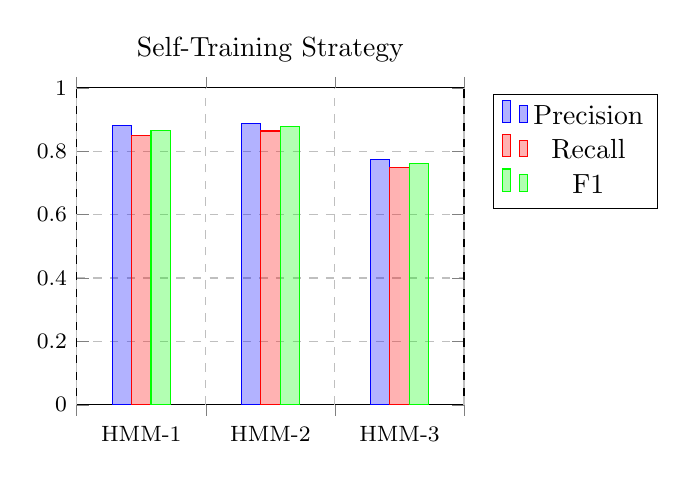
\begin{tikzpicture}
      \pgfplotsset{small}
      \begin{axis}[
        title={Self-Training Strategy},
        xmin=0.5, xmax=3.5,
        ymin=0, ymax=1,
        xticklabels={HMM-1,HMM-2,HMM-3},
        xtick={1,...,3},
        ytick={0,0.2,...,1},
        ybar=0pt,
        bar width=7pt,
        xtick distance=1,
        xtick style={
            /pgfplots/major tick length=0pt,
        },
        extra x ticks={-0.5,0.5,...,5.5},
        extra x tick labels=\empty,
        extra x tick style={
            grid=major,
            xtick style={
                /pgfplots/major tick length=4pt,
            },
        },
        ymajorgrids=true,
        grid style=dashed,
        % legend pos=north east,
	legend style={at={(1.5,0.8)},anchor=east},
      ]

      \addplot[ybar, color=blue, fill=blue, fill opacity=0.3,] coordinates {
        (1,0.880)(2,0.888)(3,0.774)
      };
      \addplot[ybar, color=red, fill=red, fill opacity=0.3,] coordinates {
        (1,0.850)(2,0.864)(3,0.750)
      };
      \addplot[ybar, color=green, fill=green, fill opacity=0.3,] coordinates {
        (1,0.865)(2,0.879)(3,0.762)
      };
      \legend{Precision, Recall, F1};
       
      \end{axis}
    \end{tikzpicture}

    \caption{Hidden Markov Models trained with the features in Group A and Group B.}
    \label{fig:hmm_self_training}
  \end{center}
\end{figure}

\begin{table}[h]
  \small
  \begin{center}
    \begin{tabular}{ lllllll }
      \toprule
      \multirow{2}{*}{Model} & \multicolumn{3}{c}{Validation} & \multicolumn{3}{c}{Test} \\
                             & \multicolumn{1}{c}{P} & \multicolumn{1}{c}{R} & \multicolumn{1}{c}{F1}
                             & \multicolumn{1}{c}{P} & \multicolumn{1}{c}{R} & \multicolumn{1}{c}{F1} \\
      \midrule
      \midrule
      HMM-1                           & 0.693 & 0.581 & 0.632 & 0.637 & 0.458 & 0.533 \\
      HMM-2                           & 0.703 & 0.630 & 0.665 & 0.653 & 0.527 & 0.583 \\
      HMM-3                           & 0.616 & 0.618 & 0.617 & 0.551 & 0.468 & 0.506 \\
      HMM-1 (Group A)                 & 0.813 & 0.816 & 0.814 & 0.819 & 0.792 & 0.805 \\
      HMM-2 (Group A)                 & 0.787 & 0.820 & 0.803 & 0.823 & 0.802 & 0.812 \\
      HMM-3 (Group A)                 & 0.774 & 0.816 & 0.795 & 0.812 & 0.785 & 0.798 \\
      HMM-1 (Group B)                 & 0.730 & 0.714 & 0.722 & 0.826 & 0.684 & 0.748 \\
      HMM-2 (Group B)                 & 0.720 & 0.710 & 0.715 & 0.820 & 0.724 & 0.769 \\
      HMM-3 (Group B)                 & 0.721 & 0.702 & 0.711 & 0.791 & 0.667 & 0.724 \\
      HMM-1 (Group A) + Self-Training & 0.752 & 0.876 & 0.810 & 0.880 & 0.851 & 0.865 \\
      HMM-2 (Group A) + Self-Training & 0.784 & 0.892 & 0.835 & \textbf{0.888} & 0.864 & \textbf{0.879} \\
      HMM-3 (Group A) + Self-Training & 0.789 & 0.891 & 0.837 & 0.774 & 0.750 & 0.762 \\
      HMM-1 (Group B) + Self-Training & 0.747 & 0.906 & 0.819 & 0.866 & 0.867 & 0.866 \\
      HMM-2 (Group B) + Self-Training & 0.771 & 0.912 & 0.835 & 0.885 & \textbf{0.869} & 0.877 \\
      HMM-3 (Group B) + Self-Training & 0.788 & 0.917 & 0.847 & 0.826 & 0.803 & 0.814 \\
      \bottomrule
    \end{tabular}
  \end{center}
  \caption{All \textit{Hidden Markov Models}}
  \label{tab:hmm_results}
\end{table}


\section{Conditional Random Fields}

Linear \textit{Chain Conditional Random Fields} provide a much more flexible way to incorporate 
features in our model in comparison to \textit{Hidden Markov Models}. When considering the application
of this class of models to the \textit{Name Extraction Task}, we want to understand how the feature
selection impacts the performance of our model and if pretrained word embeddings can help improving
its performance.

\subsection{No Features}

Figure~\ref{fig:crf_without_features} shows a comparison between the \textit{Maximum Entropy Model}
that assumes label independence, the best \textit{Hidden Markov Model} from the previous section without features
and a \textit{Linear Chain CRF} at the name extraction task. The \textit{Maxent} and \textit{CRF} use 
one-hot representations of the words. Also, different from \textit{HMMs} the discriminative models resort to numerical 
optimization methods, therefore their parameters may vary between different runs, so we present the average result 
for each measure over five runs.

\begin{figure}[h!]
  \begin{center}
    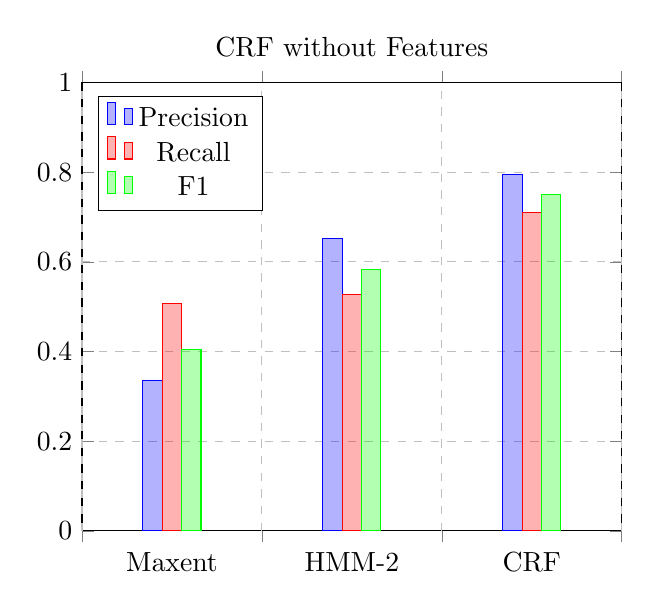
\begin{tikzpicture}
      \begin{axis}[
        title={CRF without Features},
        xmin=0.5, xmax=3.5,
        ymin=0, ymax=1,
        xticklabels={Maxent,HMM-2,CRF},
        xtick={1,...,3},
        ytick={0,0.2,...,1},
        ybar=0pt,
        bar width=7pt,
        xtick distance=1,
        xtick style={
            /pgfplots/major tick length=0pt,
        },
        extra x ticks={-0.5,0.5,...,5.5},
        extra x tick labels=\empty,
        extra x tick style={
            grid=major,
            xtick style={
                /pgfplots/major tick length=4pt,
            },
        },
        ymajorgrids=true,
        grid style=dashed,
        legend pos=north west,
      ]

      \addplot[ybar, color=blue, fill=blue, fill opacity=0.3,] coordinates {
        (1,0.335)(2,0.653)(3,0.795)
      };
      \addplot[ybar, color=red, fill=red, fill opacity=0.3,] coordinates {
        (1,0.508)(2,0.527)(3,0.710)
      };
      \addplot[ybar, color=green, fill=green, fill opacity=0.3,] coordinates {
        (1,0.404)(2,0.583)(3,0.750)
      };
      \legend{Precision, Recall, F1};
       
      \end{axis}
    \end{tikzpicture}
    \caption{
      Performance of the Maximum Entropy classifier, second-order Hidden Markov Models and 
      Linear Chain CRFs without features besides the current word on the test set of the NER on HTML dataset.
    }
    \label{fig:hmm_no_features}
  \end{center}
\end{figure}

The \textit{CRF} model shows a significant improvement in comparison to the other models that used no features,
achieving an F1-score of 0.750. Next we proceed to understand if the addition of features can improve this
performance further.


\subsection{Feature Selection}

To allow comparison between the \textit{HMMs} from the last section we consider \textit{CRFs} using features
from \textit{Group A} and \textit{Group B}. Figure~\ref{fig:} shows a comparison between the best \textit{HMM}
for each group of features and the \textit{CRF}.

\begin{figure}[h!]
  \begin{center}
    \tiny
    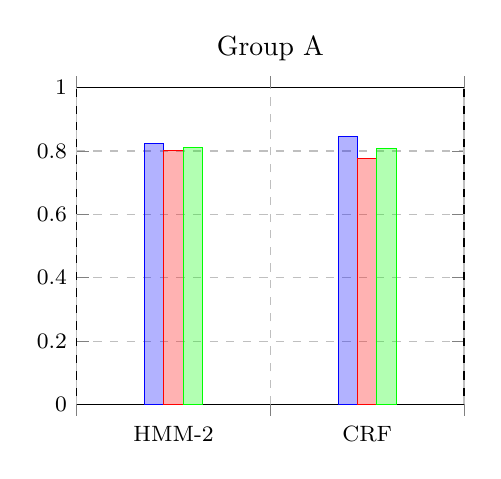
\begin{tikzpicture}
      \pgfplotsset{small}
      \begin{axis}[
        title={Group A},
        xmin=0.5, xmax=2.5,
        ymin=0, ymax=1,
        xticklabels={HMM-2,CRF},
        xtick={1,...,2},
        ytick={0,0.2,...,1},
        ybar=0pt,
        bar width=7pt,
        xtick distance=1,
        xtick style={
            /pgfplots/major tick length=0pt,
        },
        extra x ticks={-0.5,0.5,...,5.5},
        extra x tick labels=\empty,
        extra x tick style={
            grid=major,
            xtick style={
                /pgfplots/major tick length=4pt,
            },
        },
        ymajorgrids=true,
        grid style=dashed,
      ]

      \addplot[ybar, color=blue, fill=blue, fill opacity=0.3,] coordinates {
        (1,0.823)(2,0.845)
      };
      \addplot[ybar, color=red, fill=red, fill opacity=0.3,] coordinates {
        (1,0.802)(2,0.775)
      };
      \addplot[ybar, color=green, fill=green, fill opacity=0.3,] coordinates {
        (1,0.812)(2,0.808)
      };
      \legend{};
       
      \end{axis}
    \end{tikzpicture}
    ~
    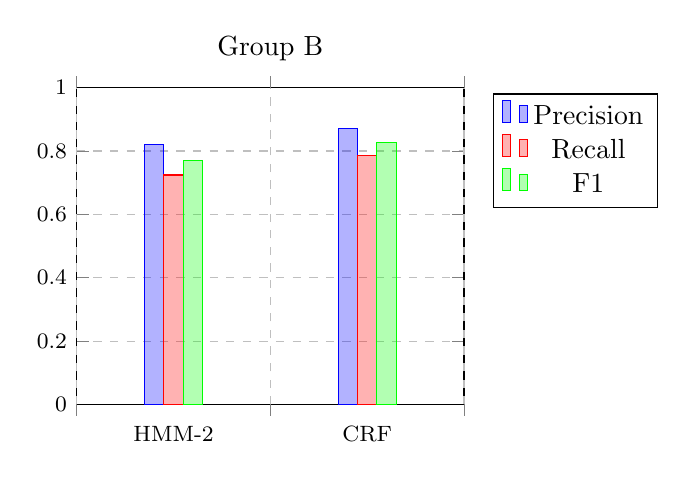
\begin{tikzpicture}
      \pgfplotsset{small}
      \begin{axis}[
        title={Group B},
        xmin=0.5, xmax=2.5,
        ymin=0, ymax=1,
        xticklabels={HMM-2,CRF},
        xtick={1,...,2},
        ytick={0,0.2,...,1},
        ybar=0pt,
        bar width=7pt,
        xtick distance=1,
        xtick style={
            /pgfplots/major tick length=0pt,
        },
        extra x ticks={-0.5,0.5,...,5.5},
        extra x tick labels=\empty,
        extra x tick style={
            grid=major,
            xtick style={
                /pgfplots/major tick length=4pt,
            },
        },
        ymajorgrids=true,
        grid style=dashed,
        % legend pos=north east,
	legend style={at={(1.5,0.8)},anchor=east},
      ]

      \addplot[ybar, color=blue, fill=blue, fill opacity=0.3,] coordinates {
        (1,0.820)(2,0.870)
      };
      \addplot[ybar, color=red, fill=red, fill opacity=0.3,] coordinates {
        (1,0.724)(2,0.786)
      };
      \addplot[ybar, color=green, fill=green, fill opacity=0.3,] coordinates {
        (1,0.769)(2,0.826)
      };
      \legend{Precision, Recall, F1};
       
      \end{axis}
    \end{tikzpicture}

    \caption{Linear Chain Conditional Random Fields trained with the features in Group A and Group B.}
    \label{fig:crf_all_features}
  \end{center}
\end{figure}

As expected, the \textit{CRF} is more robust to variations in the feature selection. It performs
similar to the second-order \textit{HMM} in \textit{Group A} and slightly better in \textit{Group B}, though
it tends towards an increase in precision rather than recall. The \textit{CRF} is marginally better than
the \textit{HMM}, however, when we consider the self-trained \textit{HMM-2}, it still shows a better overall 
performance. There are two things that could still be tried to improve the \textit{CRF} performance. First,
the \textit{CRF} allows for a more flexible feature selection, so we could try adding any imaginable feature,
since feature correlation is not impeditive in this case. Second, we could try developing a self-training 
strategy for \textit{CRFs} similar to the one employed on \textit{HMMs}. However, \textit{Neural Networks} 
showed a superior performance in many NLP tasks, so we prefered to try a \textit{Neural Network}-based approach 
next. Table~\ref{tab:crf_results} presents the detailed results for \textit{CRFs} at the name extraction
task in the validation and test sets.

\begin{table}[h]
  \small
  \begin{center}
    \begin{tabular}{ lllllll }
      \toprule
      \multirow{2}{*}{Model} & \multicolumn{3}{c}{Validation} & \multicolumn{3}{c}{Test} \\
                             & \multicolumn{1}{c}{P} & \multicolumn{1}{c}{R} & \multicolumn{1}{c}{F1}
                             & \multicolumn{1}{c}{P} & \multicolumn{1}{c}{R} & \multicolumn{1}{c}{F1} \\
      \midrule
      \midrule
      CRF                    & 0.806 & 0.805 & 0.806 & 0.795 & 0.710 & 0.750 \\
      CRF (Group A)          & 0.857 & 0.875 & 0.866 & 0.845 & 0.775 & 0.808 \\
      CRF (Group B)          & 0.881 & 0.903 & 0.892 & \textbf{0.870} & \textbf{0.786} & \textbf{0.826} \\
      \bottomrule
    \end{tabular}
  \end{center}
  \caption{All \textit{Conditional Random Fields}}
  \label{tab:crf_results}
\end{table}

\section{Neural Networks}

There are multiple \textit{Neural Network Architectures} that are suitable for solving 
\textit{Sequence Labeling} tasks. A model that has recently had remarkable success at 
solving these types of tasks is the BI-LSTM-CRF discussed in Section~\ref{sec:lstm_crf},
so we start our investigation by determining if it is also suited for the researcher
name extraction task. Additionaly, we want to determine if the CNN-based or LSTM-based
character representations can help improving the LSTM-CRF performance. We also want to
test if the Hard-Attention and Soft-Attention mechanisms for incorporating HTML structural
features provides any improvement. Finally, we want to understand if the F-score optimization
function can help controlling how much the model values precision in detriment of recall and
vice versa.


\subsection{Bi-LSTM-CRF with Glove-300 Embeddings}

One of the advantages of deep neural
networks is the fact that they can usually work without any feature engineering. 
Figure~\ref{fig:bi_lstm_crf} compares the performance of a \textit{BI-LSTM-CRF} on the test
set of the researcher name extraction task with the best \textit{HMM} and \textit{CRF} 
without features.

\begin{figure}[h!]
  \begin{center}
    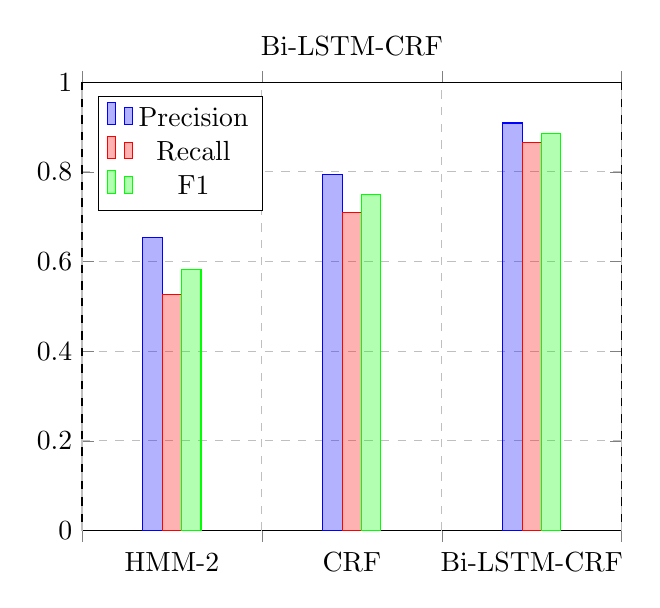
\begin{tikzpicture}
      \begin{axis}[
        title={Bi-LSTM-CRF},
        xmin=0.5, xmax=3.5,
        ymin=0, ymax=1,
        xticklabels={HMM-2,CRF,Bi-LSTM-CRF},
        xtick={1,...,3},
        ytick={0,0.2,...,1},
        ybar=0pt,
        bar width=7pt,
        xtick distance=1,
        xtick style={
            /pgfplots/major tick length=0pt,
        },
        extra x ticks={-0.5,0.5,...,5.5},
        extra x tick labels=\empty,
        extra x tick style={
            grid=major,
            xtick style={
                /pgfplots/major tick length=4pt,
            },
        },
        ymajorgrids=true,
        grid style=dashed,
        legend pos=north west,
      ]

      \addplot[ybar, color=blue, fill=blue, fill opacity=0.3,] coordinates {
        (1,0.653)(2,0.795)(3,0.909)
      };
      \addplot[ybar, color=red, fill=red, fill opacity=0.3,] coordinates {
        (1,0.527)(2,0.710)(3,0.865)
      };
      \addplot[ybar, color=green, fill=green, fill opacity=0.3,] coordinates {
        (1,0.583)(2,0.750)(3,0.886)
      };
      \legend{Precision, Recall, F1};
       
      \end{axis}
    \end{tikzpicture}
    \caption{
      Performance of the Bi-LSTM-CRF in comparison with the second-order Hidden Markov Models and 
      Linear Chain CRFs without features.
    }
    \label{fig:hmm_no_features}
  \end{center}
\end{figure}

The Bi-LSTM-CRF improves the performance of earlier models by a significant margin, though the
comparison is not completely fair, since we fed the model with Glove-300 word embeddings. However,
these pretrained embeddings are general to any language related task, so their incorporation in
does not require a lot of additional effort. Without any feature engineering, the Bi-LSTM-CRF model
already achieves an F1-score of 0.886, surpassing the best model up to this point (the HMM-2 with
self-training, which achieved 0.879 F1-score).


\subsection{Character Representations}

Morphological features can help identifying named entities. We presented in Section~\ref{sec:char_representations}
two methods for incorporating character representations in \textit{Recurrent Neural Networks}, the \textit{CNN-based}
method, and the \textit{LSTM-based} method. In Table~\ref{tab:char_reps}, we compare the performance of
\textit{CNN} and \textit{LSTM} representations with the plain \textit{Bi-LSTM-CRF}.

\begin{table}[h]
  \small
  \begin{center}
    \begin{tabular}{ lllllll }
      \toprule
      Model & Precision & Recall & F1 \\
      \midrule
      Bi-LSTM-CRF                        & 0.909 (0.008) & 0.865 (0.020) & 0.886 (0.011) \\
      Bi-LSTM-CRF + CNN chars            & 0.921 (0.006) & 0.881 (0.005) & 0.901 (0.002) \\
      Bi-LSTM-CRF + LSTM chars           & 0.920 (0.007) & 0.886 (0.031) & 0.902 (0.019) \\
      Bi-LSTM-CRF (Group B)              & 0.921 (0.008) & 0.883 (0.022) & 0.901 (0.008) \\
      Bi-LSTM-CRF (Group B) + CNN chars  & 0.922 (0.006) & 0.868 (0.033) & 0.894 (0.018) \\
      Bi-LSTM-CRF (Group B) + LSTM chars & 0.913 (0.005) & 0.855 (0.021) & 0.883 (0.012) \\
      \bottomrule
    \end{tabular}
  \end{center}
  \caption{Bi-LSTM-CRF with Character Representations}
  \label{tab:char_reps}
\end{table}

The character representations improved the \textit{F1-score} by ~1.3 points. Also, both the 
\textit{CNN-based} and the \textit{LSTM-based} representations have a similar performance, yet 
the \textit{LSTM-based} representations are slightly better, owing probably to the fact that they 
can represent prefixes and suffixes while the \textit{CNN-based} filters are position 
invariant. 

We also present the results for these models using the features from \textit{Group B}. The
addition of features improves the performance of the plain \textit{Bi-LSTM-CRF}, but hurts the 
performance of the models with character representations.


\subsection{Attention Mechanisms}

The \textit{Self-Training} strategy for \textit{HMMs} showed that there is a lot to gain
from incorporating features related to the HTML structure in our models. The hard and soft
attention mechanisms proposed in Section~\ref{sec:attention} are two ways to do that. We 
compare the performance of the \textit{Bi-LSTM-CRF} with \textit{LSTM-based} character 
representations with the same model using a Hard Attention layer and a Soft Attention 
layer in Table~\ref{tab:attention}.

\begin{table}[h]
  \small
  \begin{center}
    \begin{tabular}{ lllllll }
      \toprule
      Model & Precision & Recall & F1 \\
      \midrule
      Bi-LSTM-CRF + LSTM chars           & 0.920 (0.007) & 0.886 (0.031) & 0.902 (0.019) \\
      ... + Hard Attention               & 0.925 (0.007) & 0.890 (0.011) & 0.907 (0.005) \\
      ... + Soft Attention               & 0.884 (0.025) & 0.849 (0.021) & 0.866 (0.013) \\
      \bottomrule
    \end{tabular}
  \end{center}
  \caption{Hard and Soft Attention}
  \label{tab:attention}
\end{table}

The \textit{Hard Attention} layer improved the original model by roughly 0.5 F1-score with the
bonus of reducing variance significantly. However,
the \textit{Soft Attention} actually hurt the performance significantly, what demands further 
explanation. The reason for this is probably that the \textit{Hard Attention} only captures if
the HTML context between two tags is exactly the same, but it does not look at what is this 
context. What the \textit{Hard Attention} layer learns is essentialy how much it can trust 
predictions made for words in the same HTML context, no matter what this context is. The 
\textit{Soft Attention} layer, however, also learns features about the HTML context, so
it can learn for example to look more at words that happen inside a <div> tag. This would not 
be problematic if all documents came from the same website, however, since this is not the case,
we cannot trust specific HTML configurations to be meaningful outside the document where they
happen. This does not mean that the \textit{Soft Attention} layer is useless, but for it to grasp
abstract structural patterns that could be useful, we would probably need a much larger dataset.


\subsection{Word Embeddings}

Up to this point, all neural architectures used Glove-300 pretrained word embeddings. However, the
choice of embeddings is of great importance to the success of neural sequence models. In fact, most
recent developments to the \textit{Named Entity Recognition} models come from the incorporation of 
better word embeddings rather than from different neural architectures. We considered three sets of
pretrained word embeddings in our experiments: Glove-300, Word2Vec-300 and Elmo.

Different from Glove-300 and Word2Vec-300, which are static, Elmo embeddings are context dependent and
need to be calculated for the specific dataset. This adds significant overhead to the model training.

(SPECIFY AWS MACHINE WHICH RUN THE MODEL HERE)

Table~\ref{tab:word_embeddings} compares the performance of different sets of word embeddings in the
\textit{Bi-LSTM-CRF} model with \textit{LSTM-based} character representations.

\begin{table}[h]
  \small
  \begin{center}
    \begin{tabular}{ lllllll }
      \toprule
      Model & Precision & Recall & F1 \\
      \midrule
      Bi-LSTM-CRF + LSTM chars + Glove    & 0.920 (0.007) & 0.886 (0.031) & 0.902 (0.019) \\
      Bi-LSTM-CRF + LSTM chars + Word2Vec & 0.899 (0.011) & 0.831 (0.028) & 0.864 (0.019) \\
      Bi-LSTM-CRF + LSTM chars + Elmo     & 0.720 (0.033) & 0.885 (0.062) & 0.794 (0.043) \\
      \bottomrule
    \end{tabular}
  \end{center}
  \caption{Word Embeddings}
  \label{tab:attention}
\end{table}

As the results in Conll-2003 show, Glove-300 embeddings are superior to Word2Vec at the \textit{Named Entity Recognition}
task. However the \textit{ELMO} embeddings showed a very poor performance, contrasting to the great improvements
it showed in many NLP tasks, including NER. This is probably due to the fact that the pretrained \textit{Language Model} 
that generates the \textit{ELMO} embeddings has been trained on plain text, which is too different from the type of HTML
that we are dealing with.

\subsection{F-score Maximization}

F-score maximization

How does the precision and recall changes as we vary the alpha?



Heuristic Filtering Strategy

How much can we improve results with simple strategies like removing 
names that are smaller than two tokens and removing honorifics at the 
beginning. 



We conducted experiments to evaluate sequence labeling methods of named entity 
recognition on HTML in the context of Web data extraction using the dataset 
described in Section~\ref{sec:ner_dataset}. The tested models are described in
Table~\ref{tab:models}.







\section{Technical specifications}

All neural models were trained using mini batch Stochastic Gradient Descent over 50 epochs with batch size 10,
learning rate 0.01, momentum 0.9 and decay rate 0.05. We used early stopping \cite{Caruana2000} to select the best 
parameters, considering the F1 measure in the validation set. All neural models used 
GloVe 100-dimensional word embeddings \cite{Pennington2014} that were fine tuned during training.
In the case of NER on HTML, word embeddings work similarly to a gazetteer. Named entities 
with the same type have similar embeddings, so good word embeddings can achieve exceptional 
performance with little training and without a gazetteer. 

\begin{table}[h]
  \small
  \begin{center}
    \begin{tabular}{ ll }
      \toprule
      Model & Description \\
      \midrule
      hmm-1            & Regular HMM \\
      hmm-2            & HMM with $ k=2 $ \\
      hmm-3            & HMM with $ k=3 $ \\
      crf              & Linear chain conditional random fields \\
      bi-lstm-crf      & BI-LSTM-CRF model \\
      bi-lstm-crf-cnn  & BI-LSTM-CRF with CNN character representations \\
      bi-lstm-crf-lstm & BI-LSTM-CRF with LSTM character representations \\
      \bottomrule
    \end{tabular}
  \end{center}
  \caption{Model descriptions}
  \label{tab:models}
\end{table}

The evaluation of model performance was done through the precision, recall and 
F1 scores \cite{Rijsbergen1979}. Precision is the percentage of named entities found by 
the model that are correct. Recall is the percentage of named entities that are present
in the corpus and were found by the model. The F1 score is a composite measure that combines
precision and recall with the formula:

\begin{equation}
F1 = \frac{2 * precision * recall}{precision + recall}
\end{equation}

Named entities were only considered to be correct if they were a complete match of the 
corresponding entity in the dataset.

\section{Experiment 1: No features}

Experiment 1 aimed to evaluate the performance of sequence model with no features
besides GloVe-100 embeddings. In the case of HMMs, only the lowercase
unaccented token was used as a feature. Table \ref{tab:experiment1} 
shows the Precision (P), Recall (R), and F1-scores (F1) for this
experiment.

\begin{table}[h]
  \small
  \begin{center}
    \begin{tabular}{ lllllll }
      \toprule
      \multirow{2}{*}{Model} & \multicolumn{3}{c}{Validation} & \multicolumn{3}{c}{Test} \\
                             & \multicolumn{1}{c}{P} & \multicolumn{1}{c}{R} & \multicolumn{1}{c}{F1}
                             & \multicolumn{1}{c}{P} & \multicolumn{1}{c}{R} & \multicolumn{1}{c}{F1} \\
      \midrule
      hmm-1	       & 0.6965 & 0.5749 & 0.6299 & 0.6263 & 0.4431 & 0.5190 \\
      hmm-2	       & 0.7047 & 0.6286 & 0.6645 & 0.6480 & 0.5222 & 0.5783 \\
      hmm-3	       & 0.6127 & 0.6141 & 0.6134 & 0.5471 & 0.4634 & 0.5018 \\
      crf	       & 0.7173 & 0.6683 & 0.6920 & 0.6671 & 0.5868 & 0.6244 \\
      bi-lstm-crf      & 0.8484 & 0.9044 & 0.8755 & 0.8358 & 0.8497 & 0.8427 \\
      bi-lstm-crf-cnn  & 0.9058 & 0.9575 & 0.9309 & 0.8779 & 0.8737 & 0.8758 \\
      bi-lstm-crf-lstm & 0.9134 & 0.9435 & 0.9282 & \textbf{0.8920} & \textbf{0.8815} & \textbf{0.8867} \\
      \bottomrule
    \end{tabular}
  \end{center}
  \caption{Precision, recall and F1 in the NER on HTML dataset for models that incorporate no features}
  \label{tab:experiment1}
\end{table}

Without carefully designed features or gazetteers, HMMs and CRFs have a very 
poor performance, achieving an F1-score of only 0.5783 for HMM-2 and 0.6244 for CRF
at the test set. This is expected, since these models rely on good feature selections.

The neural models achieved high F1-scores in the test
set even with the absence of features. The plain BI-LSTM-CRF architecture improved performance 
significantly in comparison with the conventional CRF (0.8427 against 0.6244). 
Also, neural character representations boosted performance by a significant margin
reaching an F1-score of 0.8758 for CNN-based representations and 0.8867 for LSTM-based
representations. LSTM based representations were superior in modelling
morphological features, perhaps because they are able to differentiate suffixes 
and prefixes, while CNN filters are position invariant. 

The results in Experiment 1 also show that pretrained word embeddings can work 
as a kind of universal gazetteer. Words with similar embeddings are likely to 
belong to the same class. This knowledge combined with the ability to learn 
morphological features can make up for the scarcity of textual data on some 
webpages.

\section{Experiment 2: All features}

Experiment 2 aimed to evaluate the performance of sequence model with all
the features described in Table~\ref{tab:features}. In this experiment, we
also evaluate the self-training strategy for HMMs described in Section 
\ref{sssec:self_training}. The self trained HMMs are described with the 
suffix "+ST". Table \ref{tab:experiment2} shows the results for Experiment 2.

\begin{table}[h]
  \small
  \begin{center}
    \begin{tabular}{ lllllll }
      \toprule
      \multirow{2}{*}{Model} & \multicolumn{3}{c}{Validation} & \multicolumn{3}{c}{Test} \\
                             & \multicolumn{1}{c}{P} & \multicolumn{1}{c}{R} & \multicolumn{1}{c}{F1}
                             & \multicolumn{1}{c}{P} & \multicolumn{1}{c}{R} & \multicolumn{1}{c}{F1} \\
      \midrule
      hmm-1	         & 0.6061 & 0.7282 & 0.6616 & 0.7106 & 0.7633 & 0.7360 \\
      hmm-2	         & 0.6279 & 0.7550 & 0.6856 & 0.7521 & 0.7810 & 0.7663 \\
      hmm-3	         & 0.6573 & 0.7819 & 0.7142 & 0.7523 & 0.7795 & 0.7657 \\
      hmm-1+ST           & 0.7032 & 0.9077 & 0.7925 & 0.7522 & 0.8663 & 0.8052 \\
      hmm-2+ST           & 0.7321 & 0.9172 & 0.8143 & 0.7737 & 0.8789 & 0.8230 \\
      hmm-3+ST           & 0.7551 & 0.9172 & 0.8283 & 0.7961 & 0.8534 & 0.8237 \\
      crf	         & 0.9024 & 0.9049 & 0.9037 & 0.8751 & 0.8227 & 0.8481 \\
      bi-lstm-crf        & 0.9430 & 0.9530 & 0.9480 & 0.8998 & 0.8527 & 0.8756 \\
      bi-lstm-crf-cnn    & 0.9244 & 0.9715 & 0.9474 & 0.9017 & \textbf{0.8973} & \textbf{0.8995} \\
      bi-lstm-crf-lstm   & 0.9465 & 0.9692 & 0.9577 & \textbf{0.9108} & 0.8715 & 0.8907 \\
      \bottomrule
    \end{tabular}
  \end{center}
  \caption{Precision, recall and F1 in the NER on HTML dataset for models that incorporate all features}
  \label{tab:experiment2}
\end{table}

Conventional models like HMMs, and CRFs can become competitive with
the right selection of features and a good gazetteer, however they still lose
to the best neural model without features, demonstrating their inherent limitations.
HMMs that employed trigrams or quadrigrams (hmm-2, hmm-3) performed better than
regular HMMs. Also, we can see that the self-training strategy for HMMs improved 
the quality of the models significantly in all cases, boosting both precision and recall. 
This hints at the possibility to adapt this strategy to neural networks and boost
the performance of neural models on the NER on HTML task.

The neural models also improved a little with the addition of features. The plain BI-LSTM-CRF
model gets a closer performance to the models that employed neural character 
representations. It suggests that the LSTM and CNN character representations 
were able to learn at least part of the morphological features automatically in the
first experiment. So, when these features are added explicitly, the differences 
in performance between different neural models become less noticeable.


\chapter{Related Work}

% Getting simple structured information out of text.

\section{Information Extraction}

In the last 20 years, the astonishing growth of public information in the Web has 
led to the development of a number of different approaches to the problem of Web 
data extraction. Traditionally, the task was solved by designing special purpose
programs called wrappers to recognize relevant data and store records in a structured
format. These early tools varied wildly relative to their degree of automation. 

It was readily perceived that manual wrapper generation was a rather tedious and
error prone process, unsuited for large scale operations. Wrappers tend to
break frequently because they rely heavily on webpage features that can change 
often. So, in the late nineties, several authors advocated for wrapper induction, a technique 
that consists of automatically constructing wrappers from a small set of examples by 
identifying delimiters or context tokens that single out the desired attributes. 
Some remarkable wrapper induction methods are WIEN \cite{Kushmerick2000}, Soft 
Mealy \cite{Hsu1998} and STALKER \cite{Muslea1999}.

Despite being better than constructing wrappers manually, wrapper induction methods 
still suffered from a lack of expressive power and flexibility. These methods had 
trouble handling records with missing attributes or unusual structures because
patterns could only be identified if they happened at least once in the examples.

Other approaches such as NoDoSE \cite{Adelberg1998} and Debye \cite{Laender2002a} 
brought greater flexibility to wrapper induction methods by requiring a greater level 
of human interaction through graphical user interfaces. Web data extraction techniques often 
require some sort of assistance from human experts to boost accuracy. One of the main challenges 
in the field lies in determining an adequate trade-off between the degree of automation and 
the precision and recall of the data extraction tool.

To automate the task of Web data extraction completely some approaches,
such as Road Runner \cite{Crescenzi2001}, removed entirely the need for data examples.
Road Runner parses documents belonging to a same class (e.g. books on Amazon) and 
generates wrappers based on their similarities and differences, yielding comparable results 
to those obtained by wrapper induction methods. However, like previous approaches, it was 
unsuited for cross site extraction tasks because the learned rules were not general enough.

NLP based approaches aimed at extracting more general rules that could possibly
be employed over multiple websites. RAPIER \cite{Califf1999} is a method of rule
extraction that uses information such as part-of-speech tags and semantic classes from
a lexicon to derive patterns from a set of training examples. This approach is more
flexible than the wrapper induction methods, however it achieves much lower rates of 
recall and precision.

In 2002, a survey by Laender et al. \cite{Laender2002} made a thorough classification of the
early approaches with a taxonomy based on their main technology, being them: languages for
wrapper development, HTML-aware tools, NLP-based tools, Wrapper Induction Tools,
Modeling-based tools and Ontology-based tools. Some noteworthy examples from this era
are: 

\begin{itemize}
\item TSIMMIS \cite{Hammer1997} and WebOQL \cite{Arocena1999}, which are special purpose 
languages for building wrappers.

\item Road Runner \cite{Crescenzi2001}, XWRAP \cite{Liu2000} and W4F \cite{Sahuguet1999}, 
which are HTML-aware tools that infer meaningful patterns from the HTML structure.

\item RAPIER \cite{Califf1999}, SRV \cite{Freitag1998}, WHISK \cite{Soderland1999}, which 
are NLP-based tools.

\item WIEN \cite{Kushmerick2000}, Soft Mealy \cite{Hsu1998} and STALKER \cite{Muslea1999} which 
are wrapper induction methods.

\item NoDoSE \cite{Adelberg1998} and Debye \cite{Laender2002a}, which are semi supervised modeling
based tools that require some interaction with the user by means of a graphical
user interface.
\end{itemize}

In 2006, Chang et al. \cite{Chang2006} complemented the previous surveys with semi-supervised 
technologies such as Thresher \cite{Hogue2005}, IEPAD \cite{Chang2001} and 
OLERA \cite{Chang2004}. They differed from supervised 
and unsupervised methods because they either needed only a rough description of
data from users for extraction rule generation or some level of post processing
that needed user attention. The survey also mentioned newer unsupervised methods
such as DeLa \cite{Wang2003}, Exalg \cite{Arasu2003} and Depta \cite{Zhai2005}.

Most of the early information extraction systems were rule-based with either 
manual rule description or automatic rule learning from examples, thus they
suffered from a lack of flexibility when dealing with noisy and unstructured data.
Huge progress in the field of statistical learning led to the development of
statistical models that tried to solve this problem.

In 2008, Sarawagi \cite{Sarawagi2008} produced a survey that classified wrappers into
rule-based methods, statistical methods and hybrid models, bringing together 
the fields of named entity recognition, relationship extraction and information extraction. 
The rule based methods encompass most of the 
previous models. The statistical methods convert the extraction task into a token labeling 
task, identifying the target entities through the assignment of labels as in a typical 
Named Entity Recognition task. Traditionally, Hidden Markov Models \cite{Leek1997,Freitag1999}, 
Linear Chain Conditional Random Fields \cite{Lafferty2001}, and Maximum Entropy Taggers 
\cite{McCallum2000} have been the usual choice for linear sequence tagging models.
More recently, with the advancement of Natural Language Processing and Deep Learning, 
neural models outperformed previous NER methods for plain text. Huang et. al. \cite{Huang2015} introduced the 
bidirectional Long Short-Term Memory (LSTM) model with a Conditional Random Field (CRF) output layer
for NER. Ma and Hovy \cite{Ma2016} incorporated Convolutional Neural Network based character representations 
on top of the architecture. And Lample et. al. \cite{Lample2016} introduced
LSTM based character representations. 

Surveys by Ferrara et al. \cite{Ferrara2014}, Schulz et al. \cite{Schulz2016} and 
Varlamov et al. \cite{Varlamov2016} updated the previous surveys on information 
extraction methods with some interesting innovations. 
Some examples are: the Visual Box Model \cite{Krupl2005}, a data extraction system that produces 
a visualization of the webpage to exploit visual cues to identify data presented in a tabular form;
automatic wrapper adaptation \cite{Ferrara2011}, a technique that tries to reduce the cost of 
wrapper maintenance by measuring the similarity of HTML trees and adapting
wrappers to the new page structure; AutoRM \cite{Shi2015}, a method to mine
records from a single webpage by identifying similar data regions through DOM
tree analysis; Knowledge Vault \cite{Dong2014}, a method that combines different 
extraction approaches to feed a probabilistic knowledge base.

Most data extraction systems focus on extracting information from single websites
and are therefore unsuited for cross website extraction tasks. Even unsupervised
approaches that are domain independent, such as RoadRunner \cite{Crescenzi2001} 
and EXALG \cite{Arasu2003} only work well for extracting data from pages generated 
from a same template. 

A statistical approach to unsupervised domain 
independent Web data extraction was described by Zhu et al \cite{Zhu2005}. The 2D CRF 
model takes a webpage segmented into data blocks and employs a two dimensional conditional 
random field model to perform attribute labeling. The model was further improved
\cite{Zhu2006} to model record segmentation and attribute labeling as a joint task.
Some of the limitations of early unsupervised methods 
were also tackled by ObjectRunner \cite{Abdessalem2010} and AMBER \cite{Furche2012}. 
These methods work by annotating webpages automatically with regular expressions, gazetteers and 
knowledge bases. They can rectify low quality annotations and even improve the annotators
by exploring regular structures in the DOM during the record segmentation phase.

Web data extraction methods have undoubtedly improved extraordinarily, but
as pointed by Schulz et al. \cite{Schulz2016}, it is difficult to compare the results 
achieved by competing tools, and many seem to rely excessively on heuristic methods.
In that regard, the recent advancements in sequence taggers may provide more robust and
flexible extraction tools.

\section{Named Entity Recognition}

also briefly state attention and F1


\chapter{Conclusion}

Machine-learning-based sequence labeling models provide a flexible approach to Web data 
extraction, in contrast to more traditional methods. In simple cases, a neural
named entity tagger may be sufficient to solve the entire data extraction task. In 
other cases, the sequence tagger remains an important part of the web data extraction
system, as it performs attribute labeling on data records with accuracy and flexibility.

In this article, we compared the performance of different sequence models on the task of
named entity recognition on HTML, introducing a novel dataset that is publicly available. 
We found that there are two components to the most successful models: neural based character 
representations that extract morphological features automatically, and the joint modelling 
of output labels.

We showed that a BI-LSTM-CRF neural network with LSTM-based character representations can 
be employed effectively to solve a web data extraction task, achieving an F1-score of 
0.8867 with no feature engineering on the faculty listings dataset.

The effective recognition of named entities on HTML is an essential step in most general 
Web data extraction methods. The accuracy achieved by deep neural architectures even
on webpages that are very different from the plain text for which these architectures 
were initially designed shows the potential for a truly flexible approach to cross domain 
web data extraction.


\ppgccbibliography{bibfile}


\begin{appendices}
\label{app:html_segmenter}

\chapter{HTML sentence segmenter}

Lorem ipsum dolor.

% \chapter{Outro ap�ndice}
% 
% \dummytxta
% 
\end{appendices}
% 
% 
% \begin{attachments}
% 
% % Para cada anexo, um \chapter
% \chapter{Um anexo}
% 
% \dummytxta
% 
% \chapter{Outro anexo}
% 
% \dummytxta
% \end{attachments}


\end{document}
